\documentclass[twoside]{book}

% Packages required by doxygen
\usepackage{fixltx2e}
\usepackage{calc}
\usepackage{doxygen}
\usepackage[export]{adjustbox} % also loads graphicx
\usepackage{graphicx}
\usepackage[utf8]{inputenc}
\usepackage{makeidx}
\usepackage{multicol}
\usepackage{multirow}
\PassOptionsToPackage{warn}{textcomp}
\usepackage{textcomp}
\usepackage[nointegrals]{wasysym}
\usepackage[table]{xcolor}

% NLS support packages
\usepackage{polski}
\usepackage[T1]{fontenc}

% Font selection
\usepackage[T1]{fontenc}
\usepackage[scaled=.90]{helvet}
\usepackage{courier}
\usepackage{amssymb}
\usepackage{sectsty}
\renewcommand{\familydefault}{\sfdefault}
\allsectionsfont{%
  \fontseries{bc}\selectfont%
  \color{darkgray}%
}
\renewcommand{\DoxyLabelFont}{%
  \fontseries{bc}\selectfont%
  \color{darkgray}%
}
\newcommand{\+}{\discretionary{\mbox{\scriptsize$\hookleftarrow$}}{}{}}

% Page & text layout
\usepackage{geometry}
\geometry{%
  a4paper,%
  top=2.5cm,%
  bottom=2.5cm,%
  left=2.5cm,%
  right=2.5cm%
}
\tolerance=750
\hfuzz=15pt
\hbadness=750
\setlength{\emergencystretch}{15pt}
\setlength{\parindent}{0cm}
\setlength{\parskip}{3ex plus 2ex minus 2ex}
\makeatletter
\renewcommand{\paragraph}{%
  \@startsection{paragraph}{4}{0ex}{-1.0ex}{1.0ex}{%
    \normalfont\normalsize\bfseries\SS@parafont%
  }%
}
\renewcommand{\subparagraph}{%
  \@startsection{subparagraph}{5}{0ex}{-1.0ex}{1.0ex}{%
    \normalfont\normalsize\bfseries\SS@subparafont%
  }%
}
\makeatother

% Headers & footers
\usepackage{fancyhdr}
\pagestyle{fancyplain}
\fancyhead[LE]{\fancyplain{}{\bfseries\thepage}}
\fancyhead[CE]{\fancyplain{}{}}
\fancyhead[RE]{\fancyplain{}{\bfseries\leftmark}}
\fancyhead[LO]{\fancyplain{}{\bfseries\rightmark}}
\fancyhead[CO]{\fancyplain{}{}}
\fancyhead[RO]{\fancyplain{}{\bfseries\thepage}}
\fancyfoot[LE]{\fancyplain{}{}}
\fancyfoot[CE]{\fancyplain{}{}}
\fancyfoot[RE]{\fancyplain{}{\bfseries\scriptsize Wygenerowano przez Doxygen }}
\fancyfoot[LO]{\fancyplain{}{\bfseries\scriptsize Wygenerowano przez Doxygen }}
\fancyfoot[CO]{\fancyplain{}{}}
\fancyfoot[RO]{\fancyplain{}{}}
\renewcommand{\footrulewidth}{0.4pt}
\renewcommand{\chaptermark}[1]{%
  \markboth{#1}{}%
}
\renewcommand{\sectionmark}[1]{%
  \markright{\thesection\ #1}%
}

% Indices & bibliography
\usepackage{natbib}
\usepackage[titles]{tocloft}
\setcounter{tocdepth}{3}
\setcounter{secnumdepth}{5}
\makeindex

% Custom commands
\newcommand{\clearemptydoublepage}{%
  \newpage{\pagestyle{empty}\cleardoublepage}%
}

\usepackage{caption}
\captionsetup{labelsep=space,justification=centering,font={bf},singlelinecheck=off,skip=4pt,position=top}

%===== C O N T E N T S =====

\begin{document}

% Titlepage & ToC
\pagenumbering{alph}
\begin{titlepage}
\vspace*{7cm}
\begin{center}%
{\Large szkola2 }\\
\vspace*{1cm}
{\large Wygenerowano przez Doxygen 1.8.13}\\
\end{center}
\end{titlepage}
\clearemptydoublepage
\pagenumbering{roman}
\tableofcontents
\clearemptydoublepage
\pagenumbering{arabic}

%--- Begin generated contents ---
\chapter{Indeks hierarchiczny}
\section{Hierarchia klas}
Ta lista dziedziczenia posortowana jest z grubsza, choć nie całkowicie, alfabetycznie\+:\begin{DoxyCompactList}
\item \contentsline{section}{Aula}{\pageref{class_aula}}{}
\item \contentsline{section}{Budynek\+Edukacyjny}{\pageref{class_budynek_edukacyjny}}{}
\begin{DoxyCompactList}
\item \contentsline{section}{Szkola}{\pageref{class_szkola}}{}
\begin{DoxyCompactList}
\item \contentsline{section}{Ponadgimnazjalna}{\pageref{class_ponadgimnazjalna}}{}
\end{DoxyCompactList}
\item \contentsline{section}{Uczelnia}{\pageref{class_uczelnia}}{}
\end{DoxyCompactList}
\item \contentsline{section}{Dziekanat}{\pageref{class_dziekanat}}{}
\item \contentsline{section}{Sala}{\pageref{class_sala}}{}
\item \contentsline{section}{Sekretariat}{\pageref{class_sekretariat}}{}
\end{DoxyCompactList}

\chapter{Indeks klas}
\section{Lista klas}
Tutaj znajdują się klasy, struktury, unie i interfejsy wraz z ich krótkimi opisami\+:\begin{DoxyCompactList}
\item\contentsline{section}{\textbf{ Aula} \\*Klasa \doxyref{Aula}{str.}{class_aula} -\/ podobiekt klasy \doxyref{Uczelnia}{str.}{class_uczelnia} }{\pageref{class_aula}}{}
\item\contentsline{section}{\textbf{ Budynek\+Edukacyjny} \\*Klasa abstrakcyjna }{\pageref{class_budynek_edukacyjny}}{}
\item\contentsline{section}{\textbf{ Dziekanat} \\*Klasa \doxyref{Dziekanat}{str.}{class_dziekanat} -\/ podobiekt klasy \doxyref{Uczelnia}{str.}{class_uczelnia} }{\pageref{class_dziekanat}}{}
\item\contentsline{section}{\textbf{ Ponadgimnazjalna} \\*Klasa \doxyref{Ponadgimnazjalna}{str.}{class_ponadgimnazjalna}, dziedziczy po klasie \doxyref{Szkola}{str.}{class_szkola} }{\pageref{class_ponadgimnazjalna}}{}
\item\contentsline{section}{\textbf{ Sala} \\*Klasa \doxyref{Sala}{str.}{class_sala} -\/ podobiekt do klasy \doxyref{Szkola}{str.}{class_szkola} }{\pageref{class_sala}}{}
\item\contentsline{section}{\textbf{ Sekretariat} \\*Klasa \doxyref{Sekretariat}{str.}{class_sekretariat} -\/ podobiekt do klasy \doxyref{Szkola}{str.}{class_szkola} }{\pageref{class_sekretariat}}{}
\item\contentsline{section}{\textbf{ Szkola} \\*Klasa \doxyref{Szkola}{str.}{class_szkola}, dziedziczy po klasie \doxyref{Budynek\+Edukacyjny}{str.}{class_budynek_edukacyjny} }{\pageref{class_szkola}}{}
\item\contentsline{section}{\textbf{ Uczelnia} \\*Klasa \doxyref{Uczelnia}{str.}{class_uczelnia}, dziedziczy po klasie \doxyref{Budynek\+Edukacyjny}{str.}{class_budynek_edukacyjny} }{\pageref{class_uczelnia}}{}
\end{DoxyCompactList}

\chapter{Indeks plików}
\section{Lista plików}
Tutaj znajduje się lista wszystkich plików z ich krótkimi opisami\+:\begin{DoxyCompactList}
\item\contentsline{section}{C\+:/\+Users/\+Ewa/\+Documents/\+Visual Studio 2015/\+Projects/\+Szkola2/\+Szkola2/\textbf{ Aula.\+cpp} }{\pageref{_aula_8cpp}}{}
\item\contentsline{section}{C\+:/\+Users/\+Ewa/\+Documents/\+Visual Studio 2015/\+Projects/\+Szkola2/\+Szkola2/\textbf{ Aula.\+h} }{\pageref{_aula_8h}}{}
\item\contentsline{section}{C\+:/\+Users/\+Ewa/\+Documents/\+Visual Studio 2015/\+Projects/\+Szkola2/\+Szkola2/\textbf{ Budynek\+Edukacyjny.\+cpp} }{\pageref{_budynek_edukacyjny_8cpp}}{}
\item\contentsline{section}{C\+:/\+Users/\+Ewa/\+Documents/\+Visual Studio 2015/\+Projects/\+Szkola2/\+Szkola2/\textbf{ Budynek\+Edukacyjny.\+h} }{\pageref{_budynek_edukacyjny_8h}}{}
\item\contentsline{section}{C\+:/\+Users/\+Ewa/\+Documents/\+Visual Studio 2015/\+Projects/\+Szkola2/\+Szkola2/\textbf{ Dziekanat.\+cpp} }{\pageref{_dziekanat_8cpp}}{}
\item\contentsline{section}{C\+:/\+Users/\+Ewa/\+Documents/\+Visual Studio 2015/\+Projects/\+Szkola2/\+Szkola2/\textbf{ Dziekanat.\+h} }{\pageref{_dziekanat_8h}}{}
\item\contentsline{section}{C\+:/\+Users/\+Ewa/\+Documents/\+Visual Studio 2015/\+Projects/\+Szkola2/\+Szkola2/\textbf{ Ponadgimnazjalna.\+cpp} }{\pageref{_ponadgimnazjalna_8cpp}}{}
\item\contentsline{section}{C\+:/\+Users/\+Ewa/\+Documents/\+Visual Studio 2015/\+Projects/\+Szkola2/\+Szkola2/\textbf{ Ponadgimnazjalna.\+h} }{\pageref{_ponadgimnazjalna_8h}}{}
\item\contentsline{section}{C\+:/\+Users/\+Ewa/\+Documents/\+Visual Studio 2015/\+Projects/\+Szkola2/\+Szkola2/\textbf{ program.\+cpp} }{\pageref{program_8cpp}}{}
\item\contentsline{section}{C\+:/\+Users/\+Ewa/\+Documents/\+Visual Studio 2015/\+Projects/\+Szkola2/\+Szkola2/\textbf{ Sala.\+cpp} }{\pageref{_sala_8cpp}}{}
\item\contentsline{section}{C\+:/\+Users/\+Ewa/\+Documents/\+Visual Studio 2015/\+Projects/\+Szkola2/\+Szkola2/\textbf{ Sala.\+h} }{\pageref{_sala_8h}}{}
\item\contentsline{section}{C\+:/\+Users/\+Ewa/\+Documents/\+Visual Studio 2015/\+Projects/\+Szkola2/\+Szkola2/\textbf{ Sekretariat.\+cpp} }{\pageref{_sekretariat_8cpp}}{}
\item\contentsline{section}{C\+:/\+Users/\+Ewa/\+Documents/\+Visual Studio 2015/\+Projects/\+Szkola2/\+Szkola2/\textbf{ Sekretariat.\+h} }{\pageref{_sekretariat_8h}}{}
\item\contentsline{section}{C\+:/\+Users/\+Ewa/\+Documents/\+Visual Studio 2015/\+Projects/\+Szkola2/\+Szkola2/\textbf{ Szkola.\+cpp} }{\pageref{_szkola_8cpp}}{}
\item\contentsline{section}{C\+:/\+Users/\+Ewa/\+Documents/\+Visual Studio 2015/\+Projects/\+Szkola2/\+Szkola2/\textbf{ Szkola.\+h} }{\pageref{_szkola_8h}}{}
\item\contentsline{section}{C\+:/\+Users/\+Ewa/\+Documents/\+Visual Studio 2015/\+Projects/\+Szkola2/\+Szkola2/\textbf{ Uczelnia.\+cpp} }{\pageref{_uczelnia_8cpp}}{}
\item\contentsline{section}{C\+:/\+Users/\+Ewa/\+Documents/\+Visual Studio 2015/\+Projects/\+Szkola2/\+Szkola2/\textbf{ Uczelnia.\+h} }{\pageref{_uczelnia_8h}}{}
\end{DoxyCompactList}

\chapter{Dokumentacja klas}
\section{Dokumentacja klasy Aula}
\label{class_aula}\index{Aula@{Aula}}


Klasa \doxyref{Aula}{str.}{class_aula} -\/ podobiekt klasy \doxyref{Uczelnia}{str.}{class_uczelnia}.  




{\ttfamily \#include $<$Aula.\+h$>$}

\subsection*{Metody publiczne}
\begin{DoxyCompactItemize}
\item 
\textbf{ Aula} ()
\begin{DoxyCompactList}\small\item\em Konstruktor. \end{DoxyCompactList}\item 
\textbf{ $\sim$\+Aula} ()
\begin{DoxyCompactList}\small\item\em Destruktor. \end{DoxyCompactList}\item 
void \textbf{ wyswietl\+Zawartosc} ()
\begin{DoxyCompactList}\small\item\em Funkcja umozliwiajaca wyswietlanie zawartosci auli. \end{DoxyCompactList}\end{DoxyCompactItemize}
\subsection*{Przyjaciele}
\begin{DoxyCompactItemize}
\item 
ostream \& \textbf{ operator$<$$<$} (ostream \&s, \textbf{ Aula} \&aula)
\begin{DoxyCompactList}\small\item\em operator strumieniowy $<$$<$ \end{DoxyCompactList}\item 
istream \& \textbf{ operator$>$$>$} (istream \&s, \textbf{ Aula} \&aula)
\begin{DoxyCompactList}\small\item\em operator strumieniowy $>$$>$ \end{DoxyCompactList}\end{DoxyCompactItemize}


\subsection{Opis szczegółowy}
Klasa \doxyref{Aula}{str.}{class_aula} -\/ podobiekt klasy \doxyref{Uczelnia}{str.}{class_uczelnia}. 

\subsection{Dokumentacja konstruktora i destruktora}
\mbox{\label{class_aula_a8d76c855afa3252523e4ba97535bd2db}} 
\index{Aula@{Aula}!Aula@{Aula}}
\index{Aula@{Aula}!Aula@{Aula}}
\subsubsection{Aula()}
{\footnotesize\ttfamily Aula\+::\+Aula (\begin{DoxyParamCaption}{ }\end{DoxyParamCaption})}



Konstruktor. 

\mbox{\label{class_aula_a3ad5a0c0717aa01569589b31dd851f2a}} 
\index{Aula@{Aula}!````~Aula@{$\sim$\+Aula}}
\index{````~Aula@{$\sim$\+Aula}!Aula@{Aula}}
\subsubsection{$\sim$\+Aula()}
{\footnotesize\ttfamily Aula\+::$\sim$\+Aula (\begin{DoxyParamCaption}{ }\end{DoxyParamCaption})}



Destruktor. 



\subsection{Dokumentacja funkcji składowych}
\mbox{\label{class_aula_ab6a5e2f1f4223f819709648e642cccd6}} 
\index{Aula@{Aula}!wyswietl\+Zawartosc@{wyswietl\+Zawartosc}}
\index{wyswietl\+Zawartosc@{wyswietl\+Zawartosc}!Aula@{Aula}}
\subsubsection{wyswietl\+Zawartosc()}
{\footnotesize\ttfamily void Aula\+::wyswietl\+Zawartosc (\begin{DoxyParamCaption}{ }\end{DoxyParamCaption})}



Funkcja umozliwiajaca wyswietlanie zawartosci auli. 



\subsection{Dokumentacja przyjaciół i funkcji związanych}
\mbox{\label{class_aula_a4feb487e7f3341c84013188b38984e09}} 
\index{Aula@{Aula}!operator$<$$<$@{operator$<$$<$}}
\index{operator$<$$<$@{operator$<$$<$}!Aula@{Aula}}
\subsubsection{operator$<$$<$}
{\footnotesize\ttfamily ostream\& operator$<$$<$ (\begin{DoxyParamCaption}\item[{ostream \&}]{s,  }\item[{\textbf{ Aula} \&}]{aula }\end{DoxyParamCaption})\hspace{0.3cm}{\ttfamily [friend]}}



operator strumieniowy $<$$<$ 

\mbox{\label{class_aula_adff0ed7dade5716526288ec1e16aaccb}} 
\index{Aula@{Aula}!operator$>$$>$@{operator$>$$>$}}
\index{operator$>$$>$@{operator$>$$>$}!Aula@{Aula}}
\subsubsection{operator$>$$>$}
{\footnotesize\ttfamily istream\& operator$>$$>$ (\begin{DoxyParamCaption}\item[{istream \&}]{s,  }\item[{\textbf{ Aula} \&}]{aula }\end{DoxyParamCaption})\hspace{0.3cm}{\ttfamily [friend]}}



operator strumieniowy $>$$>$ 



Dokumentacja dla tej klasy została wygenerowana z plików\+:\begin{DoxyCompactItemize}
\item 
C\+:/\+Users/\+Ewa/\+Documents/\+Visual Studio 2015/\+Projects/\+Szkola2/\+Szkola2/\textbf{ Aula.\+h}\item 
C\+:/\+Users/\+Ewa/\+Documents/\+Visual Studio 2015/\+Projects/\+Szkola2/\+Szkola2/\textbf{ Aula.\+cpp}\end{DoxyCompactItemize}

\section{Dokumentacja klasy Budynek\+Edukacyjny}
\label{class_budynek_edukacyjny}\index{Budynek\+Edukacyjny@{Budynek\+Edukacyjny}}


Klasa abstrakcyjna.  




{\ttfamily \#include $<$Budynek\+Edukacyjny.\+h$>$}

Diagram dziedziczenia dla Budynek\+Edukacyjny\begin{figure}[H]
\begin{center}
\leavevmode
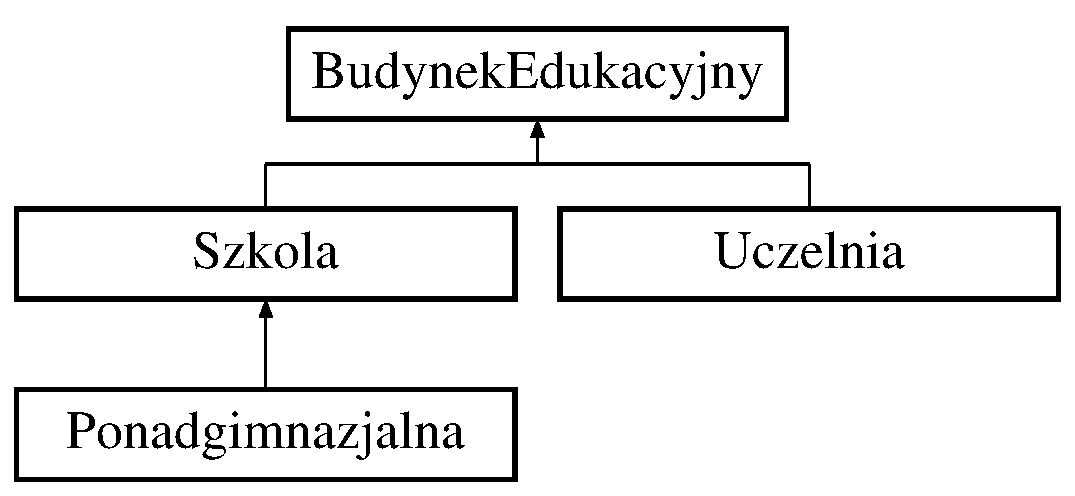
\includegraphics[height=3.000000cm]{class_budynek_edukacyjny}
\end{center}
\end{figure}
\subsection*{Metody publiczne}
\begin{DoxyCompactItemize}
\item 
\textbf{ Budynek\+Edukacyjny} ()
\begin{DoxyCompactList}\small\item\em konstruktor domyslny \end{DoxyCompactList}\item 
virtual \textbf{ $\sim$\+Budynek\+Edukacyjny} ()
\begin{DoxyCompactList}\small\item\em destruktor wirtualny \end{DoxyCompactList}\item 
void \textbf{ zapisz\+Stan} (\textbf{ Budynek\+Edukacyjny} \&budynek\+Edukacyjny, ostream \&os)
\begin{DoxyCompactList}\small\item\em Funkcja umozliwiajaca zapisywanie stanu obiektu do pliku. \end{DoxyCompactList}\item 
void \textbf{ wczytaj\+Stan} (\textbf{ Budynek\+Edukacyjny} \&budynek\+Edukacyjny, istream \&is)
\begin{DoxyCompactList}\small\item\em Funkcja umozliwiajaca odczytywanie stanu obiektu z pliku. \end{DoxyCompactList}\item 
virtual void \textbf{ wyswietl\+Stan} ()=0
\begin{DoxyCompactList}\small\item\em Funkcja wirtualna wyswietlajaca stan obiektu. \end{DoxyCompactList}\item 
virtual void \textbf{ zmien\+Liczbe\+Osob} (int nowa\+Liczba\+Osob)=0
\end{DoxyCompactItemize}
\subsection*{Przyjaciele}
\begin{DoxyCompactItemize}
\item 
ostream \& \textbf{ operator$<$$<$} (ostream \&s, \textbf{ Budynek\+Edukacyjny} \&budynek)
\begin{DoxyCompactList}\small\item\em Operator strumieniowy $<$$<$. \end{DoxyCompactList}\item 
istream \& \textbf{ operator$>$$>$} (istream \&s, \textbf{ Budynek\+Edukacyjny} \&budynek)
\begin{DoxyCompactList}\small\item\em Operator strumieniowy $>$$>$ \end{DoxyCompactList}\end{DoxyCompactItemize}


\subsection{Opis szczegółowy}
Klasa abstrakcyjna. 

\subsection{Dokumentacja konstruktora i destruktora}
\mbox{\label{class_budynek_edukacyjny_acc5537dbcd488bbbf453683ea2a587f0}} 
\index{Budynek\+Edukacyjny@{Budynek\+Edukacyjny}!Budynek\+Edukacyjny@{Budynek\+Edukacyjny}}
\index{Budynek\+Edukacyjny@{Budynek\+Edukacyjny}!Budynek\+Edukacyjny@{Budynek\+Edukacyjny}}
\subsubsection{Budynek\+Edukacyjny()}
{\footnotesize\ttfamily Budynek\+Edukacyjny\+::\+Budynek\+Edukacyjny (\begin{DoxyParamCaption}{ }\end{DoxyParamCaption})}



konstruktor domyslny 

\mbox{\label{class_budynek_edukacyjny_ace2766b8f5d6b3178267a07edac1868d}} 
\index{Budynek\+Edukacyjny@{Budynek\+Edukacyjny}!````~Budynek\+Edukacyjny@{$\sim$\+Budynek\+Edukacyjny}}
\index{````~Budynek\+Edukacyjny@{$\sim$\+Budynek\+Edukacyjny}!Budynek\+Edukacyjny@{Budynek\+Edukacyjny}}
\subsubsection{$\sim$\+Budynek\+Edukacyjny()}
{\footnotesize\ttfamily Budynek\+Edukacyjny\+::$\sim$\+Budynek\+Edukacyjny (\begin{DoxyParamCaption}{ }\end{DoxyParamCaption})\hspace{0.3cm}{\ttfamily [virtual]}}



destruktor wirtualny 



\subsection{Dokumentacja funkcji składowych}
\mbox{\label{class_budynek_edukacyjny_ac5a69c8bc9c3a96a6355b550cac15116}} 
\index{Budynek\+Edukacyjny@{Budynek\+Edukacyjny}!wczytaj\+Stan@{wczytaj\+Stan}}
\index{wczytaj\+Stan@{wczytaj\+Stan}!Budynek\+Edukacyjny@{Budynek\+Edukacyjny}}
\subsubsection{wczytaj\+Stan()}
{\footnotesize\ttfamily void Budynek\+Edukacyjny\+::wczytaj\+Stan (\begin{DoxyParamCaption}\item[{\textbf{ Budynek\+Edukacyjny} \&}]{budynek\+Edukacyjny,  }\item[{istream \&}]{is }\end{DoxyParamCaption})}



Funkcja umozliwiajaca odczytywanie stanu obiektu z pliku. 

\mbox{\label{class_budynek_edukacyjny_abb1fd21489d583814ddb2884e4402829}} 
\index{Budynek\+Edukacyjny@{Budynek\+Edukacyjny}!wyswietl\+Stan@{wyswietl\+Stan}}
\index{wyswietl\+Stan@{wyswietl\+Stan}!Budynek\+Edukacyjny@{Budynek\+Edukacyjny}}
\subsubsection{wyswietl\+Stan()}
{\footnotesize\ttfamily virtual void Budynek\+Edukacyjny\+::wyswietl\+Stan (\begin{DoxyParamCaption}{ }\end{DoxyParamCaption})\hspace{0.3cm}{\ttfamily [pure virtual]}}



Funkcja wirtualna wyswietlajaca stan obiektu. 



Implementowany w \textbf{ Szkola} \doxyref{}{str.}{class_szkola_a44e70f6bdcf477336e4c654d445a151c}, \textbf{ Uczelnia} \doxyref{}{str.}{class_uczelnia_acf5cd01d18c45a5769a87583896e79d3} i \textbf{ Ponadgimnazjalna} \doxyref{}{str.}{class_ponadgimnazjalna_a1b7a0ab77634eef40f2c13a5d65ccbfc}.

\mbox{\label{class_budynek_edukacyjny_a2ca7976a980aefccf18e2dd8533dd4c1}} 
\index{Budynek\+Edukacyjny@{Budynek\+Edukacyjny}!zapisz\+Stan@{zapisz\+Stan}}
\index{zapisz\+Stan@{zapisz\+Stan}!Budynek\+Edukacyjny@{Budynek\+Edukacyjny}}
\subsubsection{zapisz\+Stan()}
{\footnotesize\ttfamily void Budynek\+Edukacyjny\+::zapisz\+Stan (\begin{DoxyParamCaption}\item[{\textbf{ Budynek\+Edukacyjny} \&}]{budynek\+Edukacyjny,  }\item[{ostream \&}]{os }\end{DoxyParamCaption})}



Funkcja umozliwiajaca zapisywanie stanu obiektu do pliku. 

\mbox{\label{class_budynek_edukacyjny_a696551e2cc675bb42a8e82a035850c94}} 
\index{Budynek\+Edukacyjny@{Budynek\+Edukacyjny}!zmien\+Liczbe\+Osob@{zmien\+Liczbe\+Osob}}
\index{zmien\+Liczbe\+Osob@{zmien\+Liczbe\+Osob}!Budynek\+Edukacyjny@{Budynek\+Edukacyjny}}
\subsubsection{zmien\+Liczbe\+Osob()}
{\footnotesize\ttfamily virtual void Budynek\+Edukacyjny\+::zmien\+Liczbe\+Osob (\begin{DoxyParamCaption}\item[{int}]{nowa\+Liczba\+Osob }\end{DoxyParamCaption})\hspace{0.3cm}{\ttfamily [pure virtual]}}

Funkcja wirtualna zmieniajaca liczbe osob w poszczegolnych obiektach dziedziczacych po klasie \doxyref{Budynek\+Edukacyjny}{str.}{class_budynek_edukacyjny} 
\begin{DoxyParams}{Parametry}
{\em nowa\+Liczba\+Osob} & -\/ jest nowa liczba uczniow/studentow/maturzystow \\
\hline
\end{DoxyParams}


Implementowany w \textbf{ Szkola} \doxyref{}{str.}{class_szkola_aa565b62f14aeae44a2324b7e1c74147d}, \textbf{ Uczelnia} \doxyref{}{str.}{class_uczelnia_af4c8136c18a173eaf8626321e6164d35} i \textbf{ Ponadgimnazjalna} \doxyref{}{str.}{class_ponadgimnazjalna_a068d0bdb268b5e4b10d6b574681f96e3}.



\subsection{Dokumentacja przyjaciół i funkcji związanych}
\mbox{\label{class_budynek_edukacyjny_acb7de1b3048156b676e2bf8d67d5bfaf}} 
\index{Budynek\+Edukacyjny@{Budynek\+Edukacyjny}!operator$<$$<$@{operator$<$$<$}}
\index{operator$<$$<$@{operator$<$$<$}!Budynek\+Edukacyjny@{Budynek\+Edukacyjny}}
\subsubsection{operator$<$$<$}
{\footnotesize\ttfamily ostream\& operator$<$$<$ (\begin{DoxyParamCaption}\item[{ostream \&}]{s,  }\item[{\textbf{ Budynek\+Edukacyjny} \&}]{budynek }\end{DoxyParamCaption})\hspace{0.3cm}{\ttfamily [friend]}}



Operator strumieniowy $<$$<$. 

\mbox{\label{class_budynek_edukacyjny_a710e2d84c1b923f8144743db7abaa75c}} 
\index{Budynek\+Edukacyjny@{Budynek\+Edukacyjny}!operator$>$$>$@{operator$>$$>$}}
\index{operator$>$$>$@{operator$>$$>$}!Budynek\+Edukacyjny@{Budynek\+Edukacyjny}}
\subsubsection{operator$>$$>$}
{\footnotesize\ttfamily istream\& operator$>$$>$ (\begin{DoxyParamCaption}\item[{istream \&}]{s,  }\item[{\textbf{ Budynek\+Edukacyjny} \&}]{budynek }\end{DoxyParamCaption})\hspace{0.3cm}{\ttfamily [friend]}}



Operator strumieniowy $>$$>$ 



Dokumentacja dla tej klasy została wygenerowana z plików\+:\begin{DoxyCompactItemize}
\item 
C\+:/\+Users/\+Ewa/\+Documents/\+Visual Studio 2015/\+Projects/\+Szkola2/\+Szkola2/\textbf{ Budynek\+Edukacyjny.\+h}\item 
C\+:/\+Users/\+Ewa/\+Documents/\+Visual Studio 2015/\+Projects/\+Szkola2/\+Szkola2/\textbf{ Budynek\+Edukacyjny.\+cpp}\end{DoxyCompactItemize}

\section{Dokumentacja klasy Dziekanat}
\label{class_dziekanat}\index{Dziekanat@{Dziekanat}}


Klasa \doxyref{Dziekanat}{str.}{class_dziekanat} -\/ podobiekt klasy \doxyref{Uczelnia}{str.}{class_uczelnia}.  




{\ttfamily \#include $<$Dziekanat.\+h$>$}

\subsection*{Metody publiczne}
\begin{DoxyCompactItemize}
\item 
\textbf{ Dziekanat} ()
\begin{DoxyCompactList}\small\item\em Konstruktor. \end{DoxyCompactList}\item 
\textbf{ $\sim$\+Dziekanat} ()
\begin{DoxyCompactList}\small\item\em Destruktor. \end{DoxyCompactList}\item 
void \textbf{ wyswietl\+Zawartosc} ()
\item 
void \textbf{ zmien\+Liczbe\+Pan\+Z\+Dziekanatu} (int liczba\+Pan\+Z\+Dziekanatu)
\item 
void \textbf{ dziekan\+Jest} ()
\begin{DoxyCompactList}\small\item\em Funkcja zmieniajaca wartosc zmiennej czy\+Dziekan\+Tu\+Jest na true. \end{DoxyCompactList}\end{DoxyCompactItemize}
\subsection*{Przyjaciele}
\begin{DoxyCompactItemize}
\item 
ostream \& \textbf{ operator$<$$<$} (ostream \&s, \textbf{ Dziekanat} \&dziekan)
\begin{DoxyCompactList}\small\item\em operator strumieniowy $<$$<$ \end{DoxyCompactList}\item 
istream \& \textbf{ operator$>$$>$} (istream \&s, \textbf{ Dziekanat} \&dziekan)
\begin{DoxyCompactList}\small\item\em operator strumieniowy $>$$>$ \end{DoxyCompactList}\end{DoxyCompactItemize}


\subsection{Opis szczegółowy}
Klasa \doxyref{Dziekanat}{str.}{class_dziekanat} -\/ podobiekt klasy \doxyref{Uczelnia}{str.}{class_uczelnia}. 

\subsection{Dokumentacja konstruktora i destruktora}
\mbox{\label{class_dziekanat_a81b07b7d432904630e1f252d76736cdc}} 
\index{Dziekanat@{Dziekanat}!Dziekanat@{Dziekanat}}
\index{Dziekanat@{Dziekanat}!Dziekanat@{Dziekanat}}
\subsubsection{Dziekanat()}
{\footnotesize\ttfamily Dziekanat\+::\+Dziekanat (\begin{DoxyParamCaption}{ }\end{DoxyParamCaption})}



Konstruktor. 

\mbox{\label{class_dziekanat_a6bad244220341970e1059db898683e86}} 
\index{Dziekanat@{Dziekanat}!````~Dziekanat@{$\sim$\+Dziekanat}}
\index{````~Dziekanat@{$\sim$\+Dziekanat}!Dziekanat@{Dziekanat}}
\subsubsection{$\sim$\+Dziekanat()}
{\footnotesize\ttfamily Dziekanat\+::$\sim$\+Dziekanat (\begin{DoxyParamCaption}{ }\end{DoxyParamCaption})}



Destruktor. 



\subsection{Dokumentacja funkcji składowych}
\mbox{\label{class_dziekanat_afb1af21f3928ed47ac8a00c0d55801bd}} 
\index{Dziekanat@{Dziekanat}!dziekan\+Jest@{dziekan\+Jest}}
\index{dziekan\+Jest@{dziekan\+Jest}!Dziekanat@{Dziekanat}}
\subsubsection{dziekan\+Jest()}
{\footnotesize\ttfamily void Dziekanat\+::dziekan\+Jest (\begin{DoxyParamCaption}{ }\end{DoxyParamCaption})}



Funkcja zmieniajaca wartosc zmiennej czy\+Dziekan\+Tu\+Jest na true. 

\mbox{\label{class_dziekanat_add916fbcb8d862caa73a1d431bbee1a6}} 
\index{Dziekanat@{Dziekanat}!wyswietl\+Zawartosc@{wyswietl\+Zawartosc}}
\index{wyswietl\+Zawartosc@{wyswietl\+Zawartosc}!Dziekanat@{Dziekanat}}
\subsubsection{wyswietl\+Zawartosc()}
{\footnotesize\ttfamily void Dziekanat\+::wyswietl\+Zawartosc (\begin{DoxyParamCaption}{ }\end{DoxyParamCaption})}

\mbox{\label{class_dziekanat_ae3dbf1effb9c882c219b0a62d2aa9cb7}} 
\index{Dziekanat@{Dziekanat}!zmien\+Liczbe\+Pan\+Z\+Dziekanatu@{zmien\+Liczbe\+Pan\+Z\+Dziekanatu}}
\index{zmien\+Liczbe\+Pan\+Z\+Dziekanatu@{zmien\+Liczbe\+Pan\+Z\+Dziekanatu}!Dziekanat@{Dziekanat}}
\subsubsection{zmien\+Liczbe\+Pan\+Z\+Dziekanatu()}
{\footnotesize\ttfamily void Dziekanat\+::zmien\+Liczbe\+Pan\+Z\+Dziekanatu (\begin{DoxyParamCaption}\item[{int}]{liczba\+Pan\+Z\+Dziekanatu }\end{DoxyParamCaption})}

Funkcja umozliwiajaca zmiane liczby pan z dziekanatu 
\begin{DoxyParams}{Parametry}
{\em liczba\+Pan\+Z\+Dziekanatu} & okresla nowa liczbe pan \\
\hline
\end{DoxyParams}
\begin{DoxyReturn}{Zwraca}
funkcja nic nie zwraca 
\end{DoxyReturn}


\subsection{Dokumentacja przyjaciół i funkcji związanych}
\mbox{\label{class_dziekanat_a0d6451a933c737efc5a195237dc65f85}} 
\index{Dziekanat@{Dziekanat}!operator$<$$<$@{operator$<$$<$}}
\index{operator$<$$<$@{operator$<$$<$}!Dziekanat@{Dziekanat}}
\subsubsection{operator$<$$<$}
{\footnotesize\ttfamily ostream\& operator$<$$<$ (\begin{DoxyParamCaption}\item[{ostream \&}]{s,  }\item[{\textbf{ Dziekanat} \&}]{dziekan }\end{DoxyParamCaption})\hspace{0.3cm}{\ttfamily [friend]}}



operator strumieniowy $<$$<$ 

\mbox{\label{class_dziekanat_a33efe536b328cfad09ba270b61bbd54e}} 
\index{Dziekanat@{Dziekanat}!operator$>$$>$@{operator$>$$>$}}
\index{operator$>$$>$@{operator$>$$>$}!Dziekanat@{Dziekanat}}
\subsubsection{operator$>$$>$}
{\footnotesize\ttfamily istream\& operator$>$$>$ (\begin{DoxyParamCaption}\item[{istream \&}]{s,  }\item[{\textbf{ Dziekanat} \&}]{dziekan }\end{DoxyParamCaption})\hspace{0.3cm}{\ttfamily [friend]}}



operator strumieniowy $>$$>$ 



Dokumentacja dla tej klasy została wygenerowana z plików\+:\begin{DoxyCompactItemize}
\item 
C\+:/\+Users/\+Ewa/\+Documents/\+Visual Studio 2015/\+Projects/\+Szkola2/\+Szkola2/\textbf{ Dziekanat.\+h}\item 
C\+:/\+Users/\+Ewa/\+Documents/\+Visual Studio 2015/\+Projects/\+Szkola2/\+Szkola2/\textbf{ Dziekanat.\+cpp}\end{DoxyCompactItemize}

\section{Dokumentacja klasy Ponadgimnazjalna}
\label{class_ponadgimnazjalna}\index{Ponadgimnazjalna@{Ponadgimnazjalna}}


Klasa \doxyref{Ponadgimnazjalna}{str.}{class_ponadgimnazjalna}, dziedziczy po klasie \doxyref{Szkola}{str.}{class_szkola}.  




{\ttfamily \#include $<$Ponadgimnazjalna.\+h$>$}

Diagram dziedziczenia dla Ponadgimnazjalna\begin{figure}[H]
\begin{center}
\leavevmode
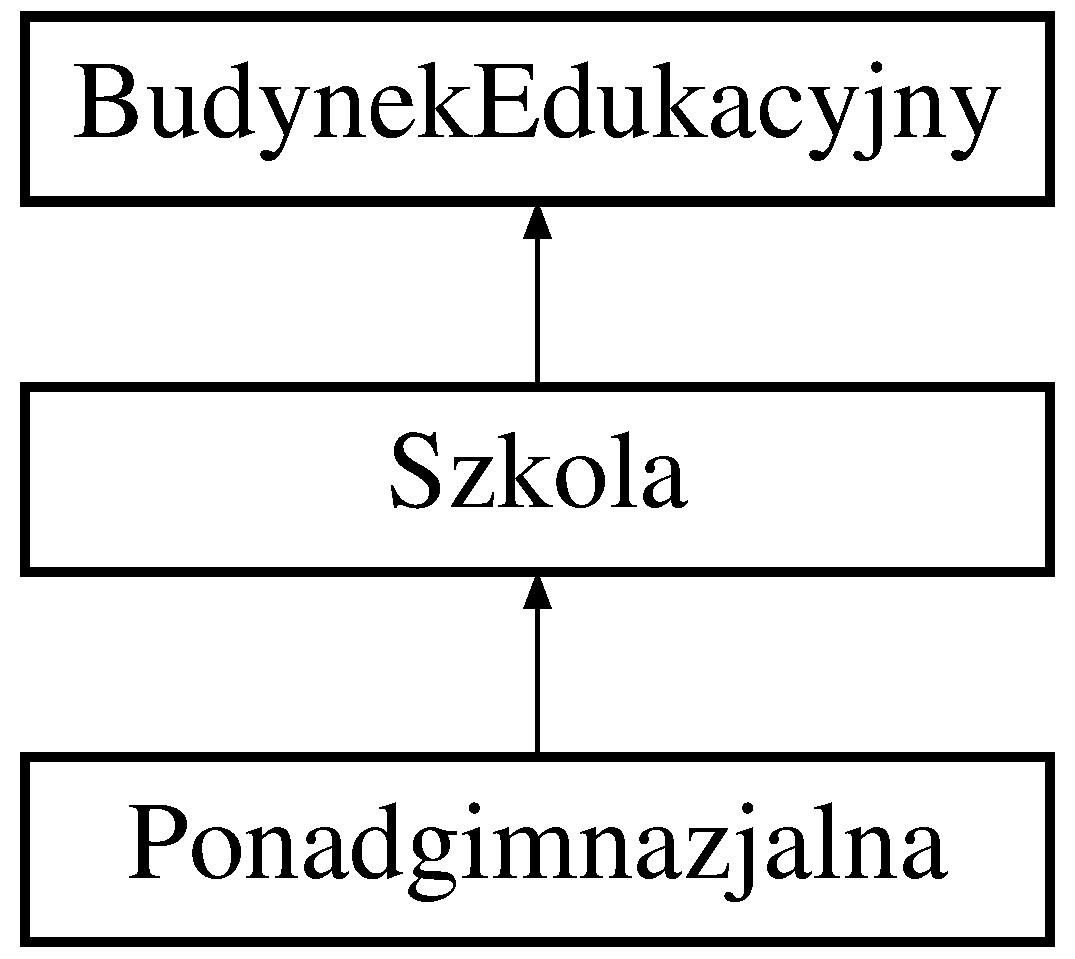
\includegraphics[height=3.000000cm]{class_ponadgimnazjalna}
\end{center}
\end{figure}
\subsection*{Metody publiczne}
\begin{DoxyCompactItemize}
\item 
\textbf{ Ponadgimnazjalna} ()
\begin{DoxyCompactList}\small\item\em Konstruktor. \end{DoxyCompactList}\item 
\textbf{ $\sim$\+Ponadgimnazjalna} ()
\begin{DoxyCompactList}\small\item\em Destruktor. \end{DoxyCompactList}\item 
void \textbf{ zapisz\+Stan} (\textbf{ Ponadgimnazjalna} \&ponadgimnazjalna, ostream \&os)
\begin{DoxyCompactList}\small\item\em Funkcja umozliwiajaca zapisywanie stanu obiektu do pliku. \end{DoxyCompactList}\item 
void \textbf{ wczytaj\+Stan} (\textbf{ Ponadgimnazjalna} \&ponadgimnazjalna, istream \&is)
\begin{DoxyCompactList}\small\item\em Funkcja umozliwiajaca odczytywanie stanu obiektu z pliku. \end{DoxyCompactList}\item 
void \textbf{ wyswietl\+Stan} ()
\begin{DoxyCompactList}\small\item\em Funkcja wirtualna wyswietlajaca stan obiektu. \end{DoxyCompactList}\item 
void \textbf{ zmien\+Liczbe\+Osob} (int nowa\+Liczba\+Osob)
\end{DoxyCompactItemize}
\subsection*{Przyjaciele}
\begin{DoxyCompactItemize}
\item 
ostream \& \textbf{ operator$<$$<$} (ostream \&s, \textbf{ Ponadgimnazjalna} \&ponadgim)
\begin{DoxyCompactList}\small\item\em operator strumieniowy $<$$<$ \end{DoxyCompactList}\item 
istream \& \textbf{ operator$>$$>$} (istream \&s, \textbf{ Ponadgimnazjalna} \&ponadgim)
\begin{DoxyCompactList}\small\item\em operator strumieniowy $>$$>$ \end{DoxyCompactList}\end{DoxyCompactItemize}
\subsection*{Dodatkowe Dziedziczone Składowe}


\subsection{Opis szczegółowy}
Klasa \doxyref{Ponadgimnazjalna}{str.}{class_ponadgimnazjalna}, dziedziczy po klasie \doxyref{Szkola}{str.}{class_szkola}. 

\subsection{Dokumentacja konstruktora i destruktora}
\mbox{\label{class_ponadgimnazjalna_ad0bfa56e49ac5112b2f36472a79fd0ff}} 
\index{Ponadgimnazjalna@{Ponadgimnazjalna}!Ponadgimnazjalna@{Ponadgimnazjalna}}
\index{Ponadgimnazjalna@{Ponadgimnazjalna}!Ponadgimnazjalna@{Ponadgimnazjalna}}
\subsubsection{Ponadgimnazjalna()}
{\footnotesize\ttfamily Ponadgimnazjalna\+::\+Ponadgimnazjalna (\begin{DoxyParamCaption}{ }\end{DoxyParamCaption})}



Konstruktor. 

\mbox{\label{class_ponadgimnazjalna_a40364cd8c83527ab7c96e64e99e0e741}} 
\index{Ponadgimnazjalna@{Ponadgimnazjalna}!````~Ponadgimnazjalna@{$\sim$\+Ponadgimnazjalna}}
\index{````~Ponadgimnazjalna@{$\sim$\+Ponadgimnazjalna}!Ponadgimnazjalna@{Ponadgimnazjalna}}
\subsubsection{$\sim$\+Ponadgimnazjalna()}
{\footnotesize\ttfamily Ponadgimnazjalna\+::$\sim$\+Ponadgimnazjalna (\begin{DoxyParamCaption}{ }\end{DoxyParamCaption})}



Destruktor. 



\subsection{Dokumentacja funkcji składowych}
\mbox{\label{class_ponadgimnazjalna_aa5994292fcdb2616c235cb06fc4c0fde}} 
\index{Ponadgimnazjalna@{Ponadgimnazjalna}!wczytaj\+Stan@{wczytaj\+Stan}}
\index{wczytaj\+Stan@{wczytaj\+Stan}!Ponadgimnazjalna@{Ponadgimnazjalna}}
\subsubsection{wczytaj\+Stan()}
{\footnotesize\ttfamily void Ponadgimnazjalna\+::wczytaj\+Stan (\begin{DoxyParamCaption}\item[{\textbf{ Ponadgimnazjalna} \&}]{ponadgimnazjalna,  }\item[{istream \&}]{is }\end{DoxyParamCaption})}



Funkcja umozliwiajaca odczytywanie stanu obiektu z pliku. 

\mbox{\label{class_ponadgimnazjalna_a1b7a0ab77634eef40f2c13a5d65ccbfc}} 
\index{Ponadgimnazjalna@{Ponadgimnazjalna}!wyswietl\+Stan@{wyswietl\+Stan}}
\index{wyswietl\+Stan@{wyswietl\+Stan}!Ponadgimnazjalna@{Ponadgimnazjalna}}
\subsubsection{wyswietl\+Stan()}
{\footnotesize\ttfamily void Ponadgimnazjalna\+::wyswietl\+Stan (\begin{DoxyParamCaption}{ }\end{DoxyParamCaption})\hspace{0.3cm}{\ttfamily [virtual]}}



Funkcja wirtualna wyswietlajaca stan obiektu. 



Implementuje \textbf{ Budynek\+Edukacyjny} \doxyref{}{str.}{class_budynek_edukacyjny_abb1fd21489d583814ddb2884e4402829}.

\mbox{\label{class_ponadgimnazjalna_a7a6714dd29b1a8d4f55fc57e61a1db01}} 
\index{Ponadgimnazjalna@{Ponadgimnazjalna}!zapisz\+Stan@{zapisz\+Stan}}
\index{zapisz\+Stan@{zapisz\+Stan}!Ponadgimnazjalna@{Ponadgimnazjalna}}
\subsubsection{zapisz\+Stan()}
{\footnotesize\ttfamily void Ponadgimnazjalna\+::zapisz\+Stan (\begin{DoxyParamCaption}\item[{\textbf{ Ponadgimnazjalna} \&}]{ponadgimnazjalna,  }\item[{ostream \&}]{os }\end{DoxyParamCaption})}



Funkcja umozliwiajaca zapisywanie stanu obiektu do pliku. 

\mbox{\label{class_ponadgimnazjalna_a068d0bdb268b5e4b10d6b574681f96e3}} 
\index{Ponadgimnazjalna@{Ponadgimnazjalna}!zmien\+Liczbe\+Osob@{zmien\+Liczbe\+Osob}}
\index{zmien\+Liczbe\+Osob@{zmien\+Liczbe\+Osob}!Ponadgimnazjalna@{Ponadgimnazjalna}}
\subsubsection{zmien\+Liczbe\+Osob()}
{\footnotesize\ttfamily void Ponadgimnazjalna\+::zmien\+Liczbe\+Osob (\begin{DoxyParamCaption}\item[{int}]{nowa\+Liczba\+Osob }\end{DoxyParamCaption})\hspace{0.3cm}{\ttfamily [virtual]}}

Funkcja wirtualna zmieniajaca liczbe osob w poszczegolnych obiektach dziedziczacych po klasie \doxyref{Budynek\+Edukacyjny}{str.}{class_budynek_edukacyjny} 
\begin{DoxyParams}{Parametry}
{\em nowa\+Liczba\+Osob} & -\/ jest nowa liczba uczniow/studentow/maturzystow \\
\hline
\end{DoxyParams}


Implementuje \textbf{ Budynek\+Edukacyjny} \doxyref{}{str.}{class_budynek_edukacyjny_a696551e2cc675bb42a8e82a035850c94}.



\subsection{Dokumentacja przyjaciół i funkcji związanych}
\mbox{\label{class_ponadgimnazjalna_a943c5cea6c4ed7ef06221e66707c693c}} 
\index{Ponadgimnazjalna@{Ponadgimnazjalna}!operator$<$$<$@{operator$<$$<$}}
\index{operator$<$$<$@{operator$<$$<$}!Ponadgimnazjalna@{Ponadgimnazjalna}}
\subsubsection{operator$<$$<$}
{\footnotesize\ttfamily ostream\& operator$<$$<$ (\begin{DoxyParamCaption}\item[{ostream \&}]{s,  }\item[{\textbf{ Ponadgimnazjalna} \&}]{ponadgim }\end{DoxyParamCaption})\hspace{0.3cm}{\ttfamily [friend]}}



operator strumieniowy $<$$<$ 

\mbox{\label{class_ponadgimnazjalna_a0b7ee50c2103c8db78c22586940f6e3b}} 
\index{Ponadgimnazjalna@{Ponadgimnazjalna}!operator$>$$>$@{operator$>$$>$}}
\index{operator$>$$>$@{operator$>$$>$}!Ponadgimnazjalna@{Ponadgimnazjalna}}
\subsubsection{operator$>$$>$}
{\footnotesize\ttfamily istream\& operator$>$$>$ (\begin{DoxyParamCaption}\item[{istream \&}]{s,  }\item[{\textbf{ Ponadgimnazjalna} \&}]{ponadgim }\end{DoxyParamCaption})\hspace{0.3cm}{\ttfamily [friend]}}



operator strumieniowy $>$$>$ 



Dokumentacja dla tej klasy została wygenerowana z plików\+:\begin{DoxyCompactItemize}
\item 
C\+:/\+Users/\+Ewa/\+Documents/\+Visual Studio 2015/\+Projects/\+Szkola2/\+Szkola2/\textbf{ Ponadgimnazjalna.\+h}\item 
C\+:/\+Users/\+Ewa/\+Documents/\+Visual Studio 2015/\+Projects/\+Szkola2/\+Szkola2/\textbf{ Ponadgimnazjalna.\+cpp}\end{DoxyCompactItemize}

\section{Dokumentacja klasy Sala}
\label{class_sala}\index{Sala@{Sala}}


Klasa \doxyref{Sala}{str.}{class_sala} -\/ podobiekt do klasy \doxyref{Szkola}{str.}{class_szkola}.  




{\ttfamily \#include $<$Sala.\+h$>$}

\subsection*{Metody publiczne}
\begin{DoxyCompactItemize}
\item 
\textbf{ Sala} ()
\begin{DoxyCompactList}\small\item\em Konstruktor. \end{DoxyCompactList}\item 
\textbf{ $\sim$\+Sala} ()
\begin{DoxyCompactList}\small\item\em Destruktor. \end{DoxyCompactList}\item 
void \textbf{ wyswietl\+Zawartosc} ()
\begin{DoxyCompactList}\small\item\em Funkcja umozliwiajaca wyswietlenie zawartosci sali. \end{DoxyCompactList}\end{DoxyCompactItemize}
\subsection*{Przyjaciele}
\begin{DoxyCompactItemize}
\item 
ostream \& \textbf{ operator$<$$<$} (ostream \&s, \textbf{ Sala} \&sala)
\begin{DoxyCompactList}\small\item\em operator strumieniowy $<$$<$ \end{DoxyCompactList}\item 
istream \& \textbf{ operator$>$$>$} (istream \&s, \textbf{ Sala} \&sala)
\begin{DoxyCompactList}\small\item\em operator strumieniowy $>$$>$ \end{DoxyCompactList}\end{DoxyCompactItemize}


\subsection{Opis szczegółowy}
Klasa \doxyref{Sala}{str.}{class_sala} -\/ podobiekt do klasy \doxyref{Szkola}{str.}{class_szkola}. 

\subsection{Dokumentacja konstruktora i destruktora}
\mbox{\label{class_sala_afcf1b7b533e776b043ce8fb13c6268ca}} 
\index{Sala@{Sala}!Sala@{Sala}}
\index{Sala@{Sala}!Sala@{Sala}}
\subsubsection{Sala()}
{\footnotesize\ttfamily Sala\+::\+Sala (\begin{DoxyParamCaption}{ }\end{DoxyParamCaption})}



Konstruktor. 

\mbox{\label{class_sala_a7e88e00e39d9cc3941636d16234dfc67}} 
\index{Sala@{Sala}!````~Sala@{$\sim$\+Sala}}
\index{````~Sala@{$\sim$\+Sala}!Sala@{Sala}}
\subsubsection{$\sim$\+Sala()}
{\footnotesize\ttfamily Sala\+::$\sim$\+Sala (\begin{DoxyParamCaption}{ }\end{DoxyParamCaption})}



Destruktor. 



\subsection{Dokumentacja funkcji składowych}
\mbox{\label{class_sala_a0b00333c8ffb56aec15edb78c1e54c5d}} 
\index{Sala@{Sala}!wyswietl\+Zawartosc@{wyswietl\+Zawartosc}}
\index{wyswietl\+Zawartosc@{wyswietl\+Zawartosc}!Sala@{Sala}}
\subsubsection{wyswietl\+Zawartosc()}
{\footnotesize\ttfamily void Sala\+::wyswietl\+Zawartosc (\begin{DoxyParamCaption}{ }\end{DoxyParamCaption})}



Funkcja umozliwiajaca wyswietlenie zawartosci sali. 



\subsection{Dokumentacja przyjaciół i funkcji związanych}
\mbox{\label{class_sala_a6469c863bb72e329da749ac256867a2f}} 
\index{Sala@{Sala}!operator$<$$<$@{operator$<$$<$}}
\index{operator$<$$<$@{operator$<$$<$}!Sala@{Sala}}
\subsubsection{operator$<$$<$}
{\footnotesize\ttfamily ostream\& operator$<$$<$ (\begin{DoxyParamCaption}\item[{ostream \&}]{s,  }\item[{\textbf{ Sala} \&}]{sala }\end{DoxyParamCaption})\hspace{0.3cm}{\ttfamily [friend]}}



operator strumieniowy $<$$<$ 

\mbox{\label{class_sala_a123daa1cada89ad7a38d48ae4f882c91}} 
\index{Sala@{Sala}!operator$>$$>$@{operator$>$$>$}}
\index{operator$>$$>$@{operator$>$$>$}!Sala@{Sala}}
\subsubsection{operator$>$$>$}
{\footnotesize\ttfamily istream\& operator$>$$>$ (\begin{DoxyParamCaption}\item[{istream \&}]{s,  }\item[{\textbf{ Sala} \&}]{sala }\end{DoxyParamCaption})\hspace{0.3cm}{\ttfamily [friend]}}



operator strumieniowy $>$$>$ 



Dokumentacja dla tej klasy została wygenerowana z plików\+:\begin{DoxyCompactItemize}
\item 
C\+:/\+Users/\+Ewa/\+Documents/\+Visual Studio 2015/\+Projects/\+Szkola2/\+Szkola2/\textbf{ Sala.\+h}\item 
C\+:/\+Users/\+Ewa/\+Documents/\+Visual Studio 2015/\+Projects/\+Szkola2/\+Szkola2/\textbf{ Sala.\+cpp}\end{DoxyCompactItemize}

\section{Dokumentacja klasy Sekretariat}
\label{class_sekretariat}\index{Sekretariat@{Sekretariat}}


Klasa \doxyref{Sekretariat}{str.}{class_sekretariat} -\/ podobiekt do klasy \doxyref{Szkola}{str.}{class_szkola}.  




{\ttfamily \#include $<$Sekretariat.\+h$>$}

\subsection*{Metody publiczne}
\begin{DoxyCompactItemize}
\item 
\textbf{ Sekretariat} ()
\begin{DoxyCompactList}\small\item\em Konstruktor. \end{DoxyCompactList}\item 
\textbf{ $\sim$\+Sekretariat} ()
\begin{DoxyCompactList}\small\item\em Destruktor. \end{DoxyCompactList}\item 
void \textbf{ wyswietl\+Zawartosc} ()
\begin{DoxyCompactList}\small\item\em Funkcja umozliwiajaca wyswietlenie zawartosci obiektu sekretariat. \end{DoxyCompactList}\item 
void \textbf{ dodatkowe\+Pomieszczenie\+Dla\+Vice} ()
\begin{DoxyCompactList}\small\item\em Funkcja zwiekszajaca o 1 liczbe pomieszczen w sekretariacie. \end{DoxyCompactList}\item 
void \textbf{ zmien\+Liczbe\+Sekretarek} (int liczba\+Sekretarek)
\item 
void \textbf{ dyrektor\+Jest} ()
\begin{DoxyCompactList}\small\item\em Funkcja zmieniajaca wartosc zmiennej czy\+Dyrektor\+Tu\+Jest na true. \end{DoxyCompactList}\end{DoxyCompactItemize}
\subsection*{Przyjaciele}
\begin{DoxyCompactItemize}
\item 
ostream \& \textbf{ operator$<$$<$} (ostream \&s, \textbf{ Sekretariat} \&sekret)
\begin{DoxyCompactList}\small\item\em operator strumieniowy $<$$<$ \end{DoxyCompactList}\item 
istream \& \textbf{ operator$>$$>$} (istream \&s, \textbf{ Sekretariat} \&sekret)
\begin{DoxyCompactList}\small\item\em operator strumieniowy $>$$>$ \end{DoxyCompactList}\end{DoxyCompactItemize}


\subsection{Opis szczegółowy}
Klasa \doxyref{Sekretariat}{str.}{class_sekretariat} -\/ podobiekt do klasy \doxyref{Szkola}{str.}{class_szkola}. 

\subsection{Dokumentacja konstruktora i destruktora}
\mbox{\label{class_sekretariat_a53de9bee6937f620918ac637d17fd50b}} 
\index{Sekretariat@{Sekretariat}!Sekretariat@{Sekretariat}}
\index{Sekretariat@{Sekretariat}!Sekretariat@{Sekretariat}}
\subsubsection{Sekretariat()}
{\footnotesize\ttfamily Sekretariat\+::\+Sekretariat (\begin{DoxyParamCaption}{ }\end{DoxyParamCaption})}



Konstruktor. 

\mbox{\label{class_sekretariat_a4667aa3034b2cd849f0a421f661a1a43}} 
\index{Sekretariat@{Sekretariat}!````~Sekretariat@{$\sim$\+Sekretariat}}
\index{````~Sekretariat@{$\sim$\+Sekretariat}!Sekretariat@{Sekretariat}}
\subsubsection{$\sim$\+Sekretariat()}
{\footnotesize\ttfamily Sekretariat\+::$\sim$\+Sekretariat (\begin{DoxyParamCaption}{ }\end{DoxyParamCaption})}



Destruktor. 



\subsection{Dokumentacja funkcji składowych}
\mbox{\label{class_sekretariat_acac93c87f1c985b9d3cc17023feb4de6}} 
\index{Sekretariat@{Sekretariat}!dodatkowe\+Pomieszczenie\+Dla\+Vice@{dodatkowe\+Pomieszczenie\+Dla\+Vice}}
\index{dodatkowe\+Pomieszczenie\+Dla\+Vice@{dodatkowe\+Pomieszczenie\+Dla\+Vice}!Sekretariat@{Sekretariat}}
\subsubsection{dodatkowe\+Pomieszczenie\+Dla\+Vice()}
{\footnotesize\ttfamily void Sekretariat\+::dodatkowe\+Pomieszczenie\+Dla\+Vice (\begin{DoxyParamCaption}{ }\end{DoxyParamCaption})}



Funkcja zwiekszajaca o 1 liczbe pomieszczen w sekretariacie. 

\mbox{\label{class_sekretariat_a039ba55b6fddf2352787b342af5e080b}} 
\index{Sekretariat@{Sekretariat}!dyrektor\+Jest@{dyrektor\+Jest}}
\index{dyrektor\+Jest@{dyrektor\+Jest}!Sekretariat@{Sekretariat}}
\subsubsection{dyrektor\+Jest()}
{\footnotesize\ttfamily void Sekretariat\+::dyrektor\+Jest (\begin{DoxyParamCaption}{ }\end{DoxyParamCaption})}



Funkcja zmieniajaca wartosc zmiennej czy\+Dyrektor\+Tu\+Jest na true. 

\mbox{\label{class_sekretariat_ac57c1148ad8cdc0f76fd8ad1f709a92b}} 
\index{Sekretariat@{Sekretariat}!wyswietl\+Zawartosc@{wyswietl\+Zawartosc}}
\index{wyswietl\+Zawartosc@{wyswietl\+Zawartosc}!Sekretariat@{Sekretariat}}
\subsubsection{wyswietl\+Zawartosc()}
{\footnotesize\ttfamily void Sekretariat\+::wyswietl\+Zawartosc (\begin{DoxyParamCaption}{ }\end{DoxyParamCaption})}



Funkcja umozliwiajaca wyswietlenie zawartosci obiektu sekretariat. 

\mbox{\label{class_sekretariat_aa0029a488e9d782edd590531a2da518c}} 
\index{Sekretariat@{Sekretariat}!zmien\+Liczbe\+Sekretarek@{zmien\+Liczbe\+Sekretarek}}
\index{zmien\+Liczbe\+Sekretarek@{zmien\+Liczbe\+Sekretarek}!Sekretariat@{Sekretariat}}
\subsubsection{zmien\+Liczbe\+Sekretarek()}
{\footnotesize\ttfamily void Sekretariat\+::zmien\+Liczbe\+Sekretarek (\begin{DoxyParamCaption}\item[{int}]{liczba\+Sekretarek }\end{DoxyParamCaption})}

Funkcja zmieniajaca liczbe sekretarek w sekretariacie 
\begin{DoxyParams}{Parametry}
{\em liczba\+Sekretarek} & okresla nowa liczbe sekretarek \\
\hline
\end{DoxyParams}
\begin{DoxyReturn}{Zwraca}
funkcja nic nie zwraca 
\end{DoxyReturn}


\subsection{Dokumentacja przyjaciół i funkcji związanych}
\mbox{\label{class_sekretariat_aca454e954cf7fe69e8efa639ee8e3fed}} 
\index{Sekretariat@{Sekretariat}!operator$<$$<$@{operator$<$$<$}}
\index{operator$<$$<$@{operator$<$$<$}!Sekretariat@{Sekretariat}}
\subsubsection{operator$<$$<$}
{\footnotesize\ttfamily ostream\& operator$<$$<$ (\begin{DoxyParamCaption}\item[{ostream \&}]{s,  }\item[{\textbf{ Sekretariat} \&}]{sekret }\end{DoxyParamCaption})\hspace{0.3cm}{\ttfamily [friend]}}



operator strumieniowy $<$$<$ 

\mbox{\label{class_sekretariat_abb745528930b0ce605757ea9e58a29c6}} 
\index{Sekretariat@{Sekretariat}!operator$>$$>$@{operator$>$$>$}}
\index{operator$>$$>$@{operator$>$$>$}!Sekretariat@{Sekretariat}}
\subsubsection{operator$>$$>$}
{\footnotesize\ttfamily istream\& operator$>$$>$ (\begin{DoxyParamCaption}\item[{istream \&}]{s,  }\item[{\textbf{ Sekretariat} \&}]{sekret }\end{DoxyParamCaption})\hspace{0.3cm}{\ttfamily [friend]}}



operator strumieniowy $>$$>$ 



Dokumentacja dla tej klasy została wygenerowana z plików\+:\begin{DoxyCompactItemize}
\item 
C\+:/\+Users/\+Ewa/\+Documents/\+Visual Studio 2015/\+Projects/\+Szkola2/\+Szkola2/\textbf{ Sekretariat.\+h}\item 
C\+:/\+Users/\+Ewa/\+Documents/\+Visual Studio 2015/\+Projects/\+Szkola2/\+Szkola2/\textbf{ Sekretariat.\+cpp}\end{DoxyCompactItemize}

\section{Dokumentacja klasy Szkola}
\label{class_szkola}\index{Szkola@{Szkola}}


Klasa \doxyref{Szkola}{str.}{class_szkola}, dziedziczy po klasie \doxyref{Budynek\+Edukacyjny}{str.}{class_budynek_edukacyjny}.  




{\ttfamily \#include $<$Szkola.\+h$>$}

Diagram dziedziczenia dla Szkola\begin{figure}[H]
\begin{center}
\leavevmode
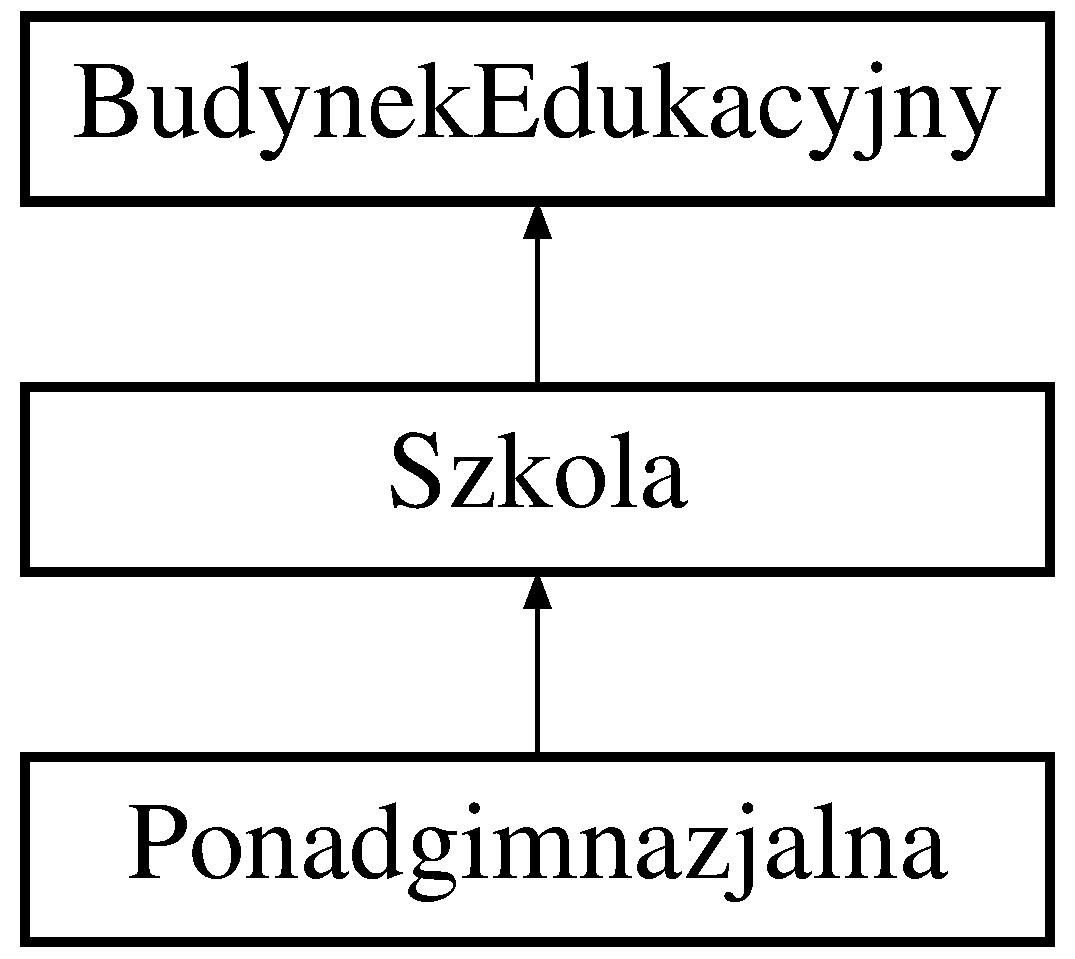
\includegraphics[height=3.000000cm]{class_szkola}
\end{center}
\end{figure}
\subsection*{Metody publiczne}
\begin{DoxyCompactItemize}
\item 
\textbf{ Szkola} ()
\begin{DoxyCompactList}\small\item\em Konstruktor domyslny. \end{DoxyCompactList}\item 
\textbf{ $\sim$\+Szkola} ()
\begin{DoxyCompactList}\small\item\em Destruktor. \end{DoxyCompactList}\item 
void \textbf{ zapisz\+Stan} (\textbf{ Szkola} \&szkola, ostream \&os)
\begin{DoxyCompactList}\small\item\em Funkcja umozliwiajaca zapisywanie stanu obiektu do pliku. \end{DoxyCompactList}\item 
void \textbf{ wczytaj\+Stan} (\textbf{ Szkola} \&szkola, istream \&is)
\begin{DoxyCompactList}\small\item\em Funkcja umozliwiajaca udczytywanie stanu obiektu z pliku. \end{DoxyCompactList}\item 
void \textbf{ wyswietl\+Stan} ()
\begin{DoxyCompactList}\small\item\em Funkcja wirtualna wyswietlajaca stan obiektu. \end{DoxyCompactList}\item 
void \textbf{ zmien\+Liczbe\+Osob} (int nowa\+Liczba\+Osob)
\item 
void \textbf{ stworz\+Sale} (int ile\+Sal)
\item 
void \textbf{ dodaj\+Sale} (\textbf{ Sala} \&sala\+Lekcyjna)
\begin{DoxyCompactList}\small\item\em Funkcja umozliwiajaca dodanie sali do szkoly. \end{DoxyCompactList}\item 
void \textbf{ pozmieniaj\+Parametry\+Sekretariatu} (int ile\+Sekretarek)
\end{DoxyCompactItemize}
\subsection*{Atrybuty chronione}
\begin{DoxyCompactItemize}
\item 
int \textbf{ liczba\+Uczniow}
\begin{DoxyCompactList}\small\item\em zmienna przechowujaca liczbe uczniow szkoly \end{DoxyCompactList}\item 
int \textbf{ liczba\+Sal}
\begin{DoxyCompactList}\small\item\em zmienna przechowujaca liczbe sal w szkole \end{DoxyCompactList}\end{DoxyCompactItemize}
\subsection*{Przyjaciele}
\begin{DoxyCompactItemize}
\item 
ostream \& \textbf{ operator$<$$<$} (ostream \&s, \textbf{ Szkola} \&szkola)
\begin{DoxyCompactList}\small\item\em Operator strumieniowy $<$$<$. \end{DoxyCompactList}\item 
istream \& \textbf{ operator$>$$>$} (istream \&s, \textbf{ Szkola} \&szkola)
\begin{DoxyCompactList}\small\item\em Operator strumieniowy $>$$>$ \end{DoxyCompactList}\end{DoxyCompactItemize}


\subsection{Opis szczegółowy}
Klasa \doxyref{Szkola}{str.}{class_szkola}, dziedziczy po klasie \doxyref{Budynek\+Edukacyjny}{str.}{class_budynek_edukacyjny}. 

\subsection{Dokumentacja konstruktora i destruktora}
\mbox{\label{class_szkola_acc1d740201e0509ab43ae6d1dae19816}} 
\index{Szkola@{Szkola}!Szkola@{Szkola}}
\index{Szkola@{Szkola}!Szkola@{Szkola}}
\subsubsection{Szkola()}
{\footnotesize\ttfamily Szkola\+::\+Szkola (\begin{DoxyParamCaption}{ }\end{DoxyParamCaption})}



Konstruktor domyslny. 

\mbox{\label{class_szkola_ac02eff91da805d8b6f9e08e0a4669155}} 
\index{Szkola@{Szkola}!````~Szkola@{$\sim$\+Szkola}}
\index{````~Szkola@{$\sim$\+Szkola}!Szkola@{Szkola}}
\subsubsection{$\sim$\+Szkola()}
{\footnotesize\ttfamily Szkola\+::$\sim$\+Szkola (\begin{DoxyParamCaption}{ }\end{DoxyParamCaption})}



Destruktor. 



\subsection{Dokumentacja funkcji składowych}
\mbox{\label{class_szkola_a0e95e2dd75a50d946f21a83c24116067}} 
\index{Szkola@{Szkola}!dodaj\+Sale@{dodaj\+Sale}}
\index{dodaj\+Sale@{dodaj\+Sale}!Szkola@{Szkola}}
\subsubsection{dodaj\+Sale()}
{\footnotesize\ttfamily void Szkola\+::dodaj\+Sale (\begin{DoxyParamCaption}\item[{\textbf{ Sala} \&}]{sala\+Lekcyjna }\end{DoxyParamCaption})}



Funkcja umozliwiajaca dodanie sali do szkoly. 

\mbox{\label{class_szkola_a16bac6c05a806c9e5077eaf447e9cf1a}} 
\index{Szkola@{Szkola}!pozmieniaj\+Parametry\+Sekretariatu@{pozmieniaj\+Parametry\+Sekretariatu}}
\index{pozmieniaj\+Parametry\+Sekretariatu@{pozmieniaj\+Parametry\+Sekretariatu}!Szkola@{Szkola}}
\subsubsection{pozmieniaj\+Parametry\+Sekretariatu()}
{\footnotesize\ttfamily void Szkola\+::pozmieniaj\+Parametry\+Sekretariatu (\begin{DoxyParamCaption}\item[{int}]{ile\+Sekretarek }\end{DoxyParamCaption})}

Funkcja zmieniajaca parametry sekretariatu wykorzystywana do sprawdzenia poprawnosci zapisu/odczytu z pliku 
\begin{DoxyParams}{Parametry}
{\em ile\+Sekretarek} & okresla nowa liczbe sekretarek, podawana przez uzytkownika \\
\hline
\end{DoxyParams}
\mbox{\label{class_szkola_a721ae2d9aa21ceab5d4eabd9f9073455}} 
\index{Szkola@{Szkola}!stworz\+Sale@{stworz\+Sale}}
\index{stworz\+Sale@{stworz\+Sale}!Szkola@{Szkola}}
\subsubsection{stworz\+Sale()}
{\footnotesize\ttfamily void Szkola\+::stworz\+Sale (\begin{DoxyParamCaption}\item[{int}]{ile\+Sal }\end{DoxyParamCaption})}

Funkcja umozliwiajaca stworzenie sal w szkole 
\begin{DoxyParams}{Parametry}
{\em ile\+Sal} & okresla ile sal ma powstac \\
\hline
\end{DoxyParams}
\begin{DoxyReturn}{Zwraca}
funkcja nic nie zwraca 
\end{DoxyReturn}
\mbox{\label{class_szkola_a448513e471b9ce17360f106c9ef823b3}} 
\index{Szkola@{Szkola}!wczytaj\+Stan@{wczytaj\+Stan}}
\index{wczytaj\+Stan@{wczytaj\+Stan}!Szkola@{Szkola}}
\subsubsection{wczytaj\+Stan()}
{\footnotesize\ttfamily void Szkola\+::wczytaj\+Stan (\begin{DoxyParamCaption}\item[{\textbf{ Szkola} \&}]{szkola,  }\item[{istream \&}]{is }\end{DoxyParamCaption})}



Funkcja umozliwiajaca udczytywanie stanu obiektu z pliku. 

\mbox{\label{class_szkola_a44e70f6bdcf477336e4c654d445a151c}} 
\index{Szkola@{Szkola}!wyswietl\+Stan@{wyswietl\+Stan}}
\index{wyswietl\+Stan@{wyswietl\+Stan}!Szkola@{Szkola}}
\subsubsection{wyswietl\+Stan()}
{\footnotesize\ttfamily void Szkola\+::wyswietl\+Stan (\begin{DoxyParamCaption}{ }\end{DoxyParamCaption})\hspace{0.3cm}{\ttfamily [virtual]}}



Funkcja wirtualna wyswietlajaca stan obiektu. 



Implementuje \textbf{ Budynek\+Edukacyjny} \doxyref{}{str.}{class_budynek_edukacyjny_abb1fd21489d583814ddb2884e4402829}.

\mbox{\label{class_szkola_aac69b456cc7836760a38dd03efa6600c}} 
\index{Szkola@{Szkola}!zapisz\+Stan@{zapisz\+Stan}}
\index{zapisz\+Stan@{zapisz\+Stan}!Szkola@{Szkola}}
\subsubsection{zapisz\+Stan()}
{\footnotesize\ttfamily void Szkola\+::zapisz\+Stan (\begin{DoxyParamCaption}\item[{\textbf{ Szkola} \&}]{szkola,  }\item[{ostream \&}]{os }\end{DoxyParamCaption})}



Funkcja umozliwiajaca zapisywanie stanu obiektu do pliku. 

\mbox{\label{class_szkola_aa565b62f14aeae44a2324b7e1c74147d}} 
\index{Szkola@{Szkola}!zmien\+Liczbe\+Osob@{zmien\+Liczbe\+Osob}}
\index{zmien\+Liczbe\+Osob@{zmien\+Liczbe\+Osob}!Szkola@{Szkola}}
\subsubsection{zmien\+Liczbe\+Osob()}
{\footnotesize\ttfamily void Szkola\+::zmien\+Liczbe\+Osob (\begin{DoxyParamCaption}\item[{int}]{nowa\+Liczba\+Osob }\end{DoxyParamCaption})\hspace{0.3cm}{\ttfamily [virtual]}}

Funkcja wirtualna zmieniajaca liczbe osob w poszczegolnych obiektach dziedziczacych po klasie \doxyref{Budynek\+Edukacyjny}{str.}{class_budynek_edukacyjny} 
\begin{DoxyParams}{Parametry}
{\em nowa\+Liczba\+Osob} & -\/ jest nowa liczba uczniow/studentow/maturzystow \\
\hline
\end{DoxyParams}


Implementuje \textbf{ Budynek\+Edukacyjny} \doxyref{}{str.}{class_budynek_edukacyjny_a696551e2cc675bb42a8e82a035850c94}.



\subsection{Dokumentacja przyjaciół i funkcji związanych}
\mbox{\label{class_szkola_add41882b5f95833d8642c9b687b36818}} 
\index{Szkola@{Szkola}!operator$<$$<$@{operator$<$$<$}}
\index{operator$<$$<$@{operator$<$$<$}!Szkola@{Szkola}}
\subsubsection{operator$<$$<$}
{\footnotesize\ttfamily ostream\& operator$<$$<$ (\begin{DoxyParamCaption}\item[{ostream \&}]{s,  }\item[{\textbf{ Szkola} \&}]{szkola }\end{DoxyParamCaption})\hspace{0.3cm}{\ttfamily [friend]}}



Operator strumieniowy $<$$<$. 

\mbox{\label{class_szkola_a5a2f94d0c0560a5fee36beba5c8501cd}} 
\index{Szkola@{Szkola}!operator$>$$>$@{operator$>$$>$}}
\index{operator$>$$>$@{operator$>$$>$}!Szkola@{Szkola}}
\subsubsection{operator$>$$>$}
{\footnotesize\ttfamily istream\& operator$>$$>$ (\begin{DoxyParamCaption}\item[{istream \&}]{s,  }\item[{\textbf{ Szkola} \&}]{szkola }\end{DoxyParamCaption})\hspace{0.3cm}{\ttfamily [friend]}}



Operator strumieniowy $>$$>$ 



\subsection{Dokumentacja atrybutów składowych}
\mbox{\label{class_szkola_a70a403bca5c564eb058e22c56ea9397b}} 
\index{Szkola@{Szkola}!liczba\+Sal@{liczba\+Sal}}
\index{liczba\+Sal@{liczba\+Sal}!Szkola@{Szkola}}
\subsubsection{liczba\+Sal}
{\footnotesize\ttfamily int Szkola\+::liczba\+Sal\hspace{0.3cm}{\ttfamily [protected]}}



zmienna przechowujaca liczbe sal w szkole 

\mbox{\label{class_szkola_a87462522c2046a383155dbde51647b1d}} 
\index{Szkola@{Szkola}!liczba\+Uczniow@{liczba\+Uczniow}}
\index{liczba\+Uczniow@{liczba\+Uczniow}!Szkola@{Szkola}}
\subsubsection{liczba\+Uczniow}
{\footnotesize\ttfamily int Szkola\+::liczba\+Uczniow\hspace{0.3cm}{\ttfamily [protected]}}



zmienna przechowujaca liczbe uczniow szkoly 



Dokumentacja dla tej klasy została wygenerowana z plików\+:\begin{DoxyCompactItemize}
\item 
C\+:/\+Users/\+Ewa/\+Documents/\+Visual Studio 2015/\+Projects/\+Szkola2/\+Szkola2/\textbf{ Szkola.\+h}\item 
C\+:/\+Users/\+Ewa/\+Documents/\+Visual Studio 2015/\+Projects/\+Szkola2/\+Szkola2/\textbf{ Szkola.\+cpp}\end{DoxyCompactItemize}

\section{Dokumentacja klasy Uczelnia}
\label{class_uczelnia}\index{Uczelnia@{Uczelnia}}


Klasa \doxyref{Uczelnia}{str.}{class_uczelnia}, dziedziczy po klasie \doxyref{Budynek\+Edukacyjny}{str.}{class_budynek_edukacyjny}.  




{\ttfamily \#include $<$Uczelnia.\+h$>$}

Diagram dziedziczenia dla Uczelnia\begin{figure}[H]
\begin{center}
\leavevmode
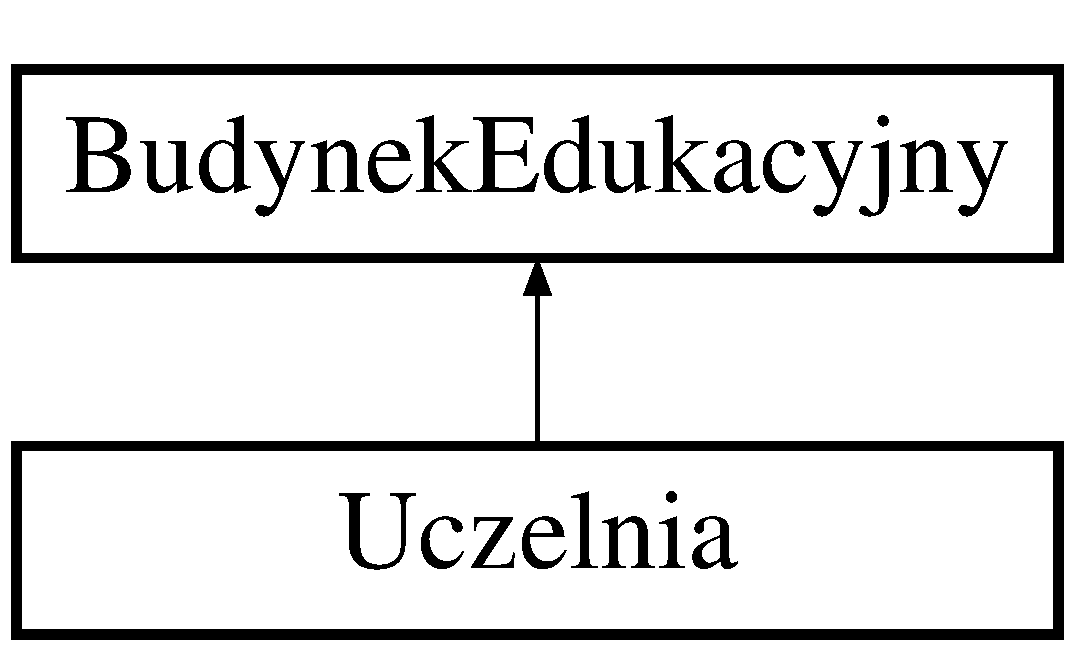
\includegraphics[height=2.000000cm]{class_uczelnia}
\end{center}
\end{figure}
\subsection*{Metody publiczne}
\begin{DoxyCompactItemize}
\item 
\textbf{ Uczelnia} ()
\begin{DoxyCompactList}\small\item\em Konstruktor. \end{DoxyCompactList}\item 
\textbf{ $\sim$\+Uczelnia} ()
\begin{DoxyCompactList}\small\item\em Destruktor. \end{DoxyCompactList}\item 
void \textbf{ zapisz\+Stan} (\textbf{ Uczelnia} \&uczelnia, ostream \&os)
\begin{DoxyCompactList}\small\item\em Funkcja umozliwiajaca zapisywanie stanu obiektu do pliku. \end{DoxyCompactList}\item 
void \textbf{ wczytaj\+Stan} (\textbf{ Uczelnia} \&uczelnia, istream \&is)
\begin{DoxyCompactList}\small\item\em Funkcja umozliwiajaca odczytywanie stanu obiektu z pliku. \end{DoxyCompactList}\item 
void \textbf{ wyswietl\+Stan} ()
\begin{DoxyCompactList}\small\item\em Funkcja wirtualna wyswietlajaca stan obiektu. \end{DoxyCompactList}\item 
void \textbf{ zmien\+Liczbe\+Osob} (int nowa\+Liczba\+Osob)
\item 
void \textbf{ pozmieniaj\+Parametry\+Dziekanatu} (int ile\+Pan\+Z\+Dziekanatu)
\begin{DoxyCompactList}\small\item\em Funkcja zmieniajaca parametry podobiektu \doxyref{Dziekanat}{str.}{class_dziekanat}. \end{DoxyCompactList}\item 
void \textbf{ stworz\+Aule} (int ile\+Auli)
\begin{DoxyCompactList}\small\item\em Funkcja umozliwiajaca stworzenie auli w uczelni. \end{DoxyCompactList}\item 
void \textbf{ dodaj\+Aule} (\textbf{ Aula} \&aula\+Wykladowa)
\begin{DoxyCompactList}\small\item\em Funkcja umozliwiajaca dodanie auli do uczelni. \end{DoxyCompactList}\end{DoxyCompactItemize}
\subsection*{Atrybuty chronione}
\begin{DoxyCompactItemize}
\item 
int \textbf{ liczba\+Studentow}
\begin{DoxyCompactList}\small\item\em zmienna przechowujaca liczbe studentow \end{DoxyCompactList}\item 
int \textbf{ liczba\+Wydzialow}
\begin{DoxyCompactList}\small\item\em zmienna przechowujaca liczbe wydzialow tej uczelni \end{DoxyCompactList}\end{DoxyCompactItemize}
\subsection*{Przyjaciele}
\begin{DoxyCompactItemize}
\item 
ostream \& \textbf{ operator$<$$<$} (ostream \&s, \textbf{ Uczelnia} \&uczelnia)
\begin{DoxyCompactList}\small\item\em operator strumieniowy $<$$<$ \end{DoxyCompactList}\item 
istream \& \textbf{ operator$>$$>$} (istream \&s, \textbf{ Uczelnia} \&uczelnia)
\begin{DoxyCompactList}\small\item\em operator strumieniowy $>$$>$ \end{DoxyCompactList}\end{DoxyCompactItemize}


\subsection{Opis szczegółowy}
Klasa \doxyref{Uczelnia}{str.}{class_uczelnia}, dziedziczy po klasie \doxyref{Budynek\+Edukacyjny}{str.}{class_budynek_edukacyjny}. 

\subsection{Dokumentacja konstruktora i destruktora}
\mbox{\label{class_uczelnia_a1d8c19ea8f3c1eb60e316658e5f85745}} 
\index{Uczelnia@{Uczelnia}!Uczelnia@{Uczelnia}}
\index{Uczelnia@{Uczelnia}!Uczelnia@{Uczelnia}}
\subsubsection{Uczelnia()}
{\footnotesize\ttfamily Uczelnia\+::\+Uczelnia (\begin{DoxyParamCaption}{ }\end{DoxyParamCaption})}



Konstruktor. 

\mbox{\label{class_uczelnia_a4d29e40e3b7a38ea0fc03309dd8db461}} 
\index{Uczelnia@{Uczelnia}!````~Uczelnia@{$\sim$\+Uczelnia}}
\index{````~Uczelnia@{$\sim$\+Uczelnia}!Uczelnia@{Uczelnia}}
\subsubsection{$\sim$\+Uczelnia()}
{\footnotesize\ttfamily Uczelnia\+::$\sim$\+Uczelnia (\begin{DoxyParamCaption}{ }\end{DoxyParamCaption})}



Destruktor. 



\subsection{Dokumentacja funkcji składowych}
\mbox{\label{class_uczelnia_aff838e457888964ab2a6c59605b496ba}} 
\index{Uczelnia@{Uczelnia}!dodaj\+Aule@{dodaj\+Aule}}
\index{dodaj\+Aule@{dodaj\+Aule}!Uczelnia@{Uczelnia}}
\subsubsection{dodaj\+Aule()}
{\footnotesize\ttfamily void Uczelnia\+::dodaj\+Aule (\begin{DoxyParamCaption}\item[{\textbf{ Aula} \&}]{aula\+Wykladowa }\end{DoxyParamCaption})}



Funkcja umozliwiajaca dodanie auli do uczelni. 

\mbox{\label{class_uczelnia_a68959f38ab2ba2809e2534297b0ee352}} 
\index{Uczelnia@{Uczelnia}!pozmieniaj\+Parametry\+Dziekanatu@{pozmieniaj\+Parametry\+Dziekanatu}}
\index{pozmieniaj\+Parametry\+Dziekanatu@{pozmieniaj\+Parametry\+Dziekanatu}!Uczelnia@{Uczelnia}}
\subsubsection{pozmieniaj\+Parametry\+Dziekanatu()}
{\footnotesize\ttfamily void Uczelnia\+::pozmieniaj\+Parametry\+Dziekanatu (\begin{DoxyParamCaption}\item[{int}]{ile\+Pan\+Z\+Dziekanatu }\end{DoxyParamCaption})}



Funkcja zmieniajaca parametry podobiektu \doxyref{Dziekanat}{str.}{class_dziekanat}. 

wykorzystywana do sprawdzenia poprawnosci zapisu/odczytu z pliku 
\begin{DoxyParams}{Parametry}
{\em ile\+Pan\+Z\+Dziekanatu} & okresla nowa liczbe pan w dziekanacie \\
\hline
\end{DoxyParams}
\mbox{\label{class_uczelnia_a6ef2e631139483a1a609df14c4689d4b}} 
\index{Uczelnia@{Uczelnia}!stworz\+Aule@{stworz\+Aule}}
\index{stworz\+Aule@{stworz\+Aule}!Uczelnia@{Uczelnia}}
\subsubsection{stworz\+Aule()}
{\footnotesize\ttfamily void Uczelnia\+::stworz\+Aule (\begin{DoxyParamCaption}\item[{int}]{ile\+Auli }\end{DoxyParamCaption})}



Funkcja umozliwiajaca stworzenie auli w uczelni. 

parametrem jest ilosc auli 
\begin{DoxyParams}{Parametry}
{\em ile\+Auli} & okresla ile podobiektow ma powstac \\
\hline
\end{DoxyParams}
\begin{DoxyReturn}{Zwraca}
funkcja nic ni zwraca 
\end{DoxyReturn}
\mbox{\label{class_uczelnia_a46339289bee2e7dccf36515f69676b4d}} 
\index{Uczelnia@{Uczelnia}!wczytaj\+Stan@{wczytaj\+Stan}}
\index{wczytaj\+Stan@{wczytaj\+Stan}!Uczelnia@{Uczelnia}}
\subsubsection{wczytaj\+Stan()}
{\footnotesize\ttfamily void Uczelnia\+::wczytaj\+Stan (\begin{DoxyParamCaption}\item[{\textbf{ Uczelnia} \&}]{uczelnia,  }\item[{istream \&}]{is }\end{DoxyParamCaption})}



Funkcja umozliwiajaca odczytywanie stanu obiektu z pliku. 

\mbox{\label{class_uczelnia_acf5cd01d18c45a5769a87583896e79d3}} 
\index{Uczelnia@{Uczelnia}!wyswietl\+Stan@{wyswietl\+Stan}}
\index{wyswietl\+Stan@{wyswietl\+Stan}!Uczelnia@{Uczelnia}}
\subsubsection{wyswietl\+Stan()}
{\footnotesize\ttfamily void Uczelnia\+::wyswietl\+Stan (\begin{DoxyParamCaption}{ }\end{DoxyParamCaption})\hspace{0.3cm}{\ttfamily [virtual]}}



Funkcja wirtualna wyswietlajaca stan obiektu. 



Implementuje \textbf{ Budynek\+Edukacyjny} \doxyref{}{str.}{class_budynek_edukacyjny_abb1fd21489d583814ddb2884e4402829}.

\mbox{\label{class_uczelnia_acaae67a14ad4965e9eb0e631be92bc47}} 
\index{Uczelnia@{Uczelnia}!zapisz\+Stan@{zapisz\+Stan}}
\index{zapisz\+Stan@{zapisz\+Stan}!Uczelnia@{Uczelnia}}
\subsubsection{zapisz\+Stan()}
{\footnotesize\ttfamily void Uczelnia\+::zapisz\+Stan (\begin{DoxyParamCaption}\item[{\textbf{ Uczelnia} \&}]{uczelnia,  }\item[{ostream \&}]{os }\end{DoxyParamCaption})}



Funkcja umozliwiajaca zapisywanie stanu obiektu do pliku. 

\mbox{\label{class_uczelnia_af4c8136c18a173eaf8626321e6164d35}} 
\index{Uczelnia@{Uczelnia}!zmien\+Liczbe\+Osob@{zmien\+Liczbe\+Osob}}
\index{zmien\+Liczbe\+Osob@{zmien\+Liczbe\+Osob}!Uczelnia@{Uczelnia}}
\subsubsection{zmien\+Liczbe\+Osob()}
{\footnotesize\ttfamily void Uczelnia\+::zmien\+Liczbe\+Osob (\begin{DoxyParamCaption}\item[{int}]{nowa\+Liczba\+Osob }\end{DoxyParamCaption})\hspace{0.3cm}{\ttfamily [virtual]}}

Funkcja wirtualna zmieniajaca liczbe osob w poszczegolnych obiektach dziedziczacych po klasie \doxyref{Budynek\+Edukacyjny}{str.}{class_budynek_edukacyjny} 
\begin{DoxyParams}{Parametry}
{\em nowa\+Liczba\+Osob} & -\/ jest nowa liczba uczniow/studentow/maturzystow \\
\hline
\end{DoxyParams}


Implementuje \textbf{ Budynek\+Edukacyjny} \doxyref{}{str.}{class_budynek_edukacyjny_a696551e2cc675bb42a8e82a035850c94}.



\subsection{Dokumentacja przyjaciół i funkcji związanych}
\mbox{\label{class_uczelnia_aaf33c9cc9b0585496b98d8d0e8558073}} 
\index{Uczelnia@{Uczelnia}!operator$<$$<$@{operator$<$$<$}}
\index{operator$<$$<$@{operator$<$$<$}!Uczelnia@{Uczelnia}}
\subsubsection{operator$<$$<$}
{\footnotesize\ttfamily ostream\& operator$<$$<$ (\begin{DoxyParamCaption}\item[{ostream \&}]{s,  }\item[{\textbf{ Uczelnia} \&}]{uczelnia }\end{DoxyParamCaption})\hspace{0.3cm}{\ttfamily [friend]}}



operator strumieniowy $<$$<$ 

\mbox{\label{class_uczelnia_a552d164e736a7caa10caed6410bf63ea}} 
\index{Uczelnia@{Uczelnia}!operator$>$$>$@{operator$>$$>$}}
\index{operator$>$$>$@{operator$>$$>$}!Uczelnia@{Uczelnia}}
\subsubsection{operator$>$$>$}
{\footnotesize\ttfamily istream\& operator$>$$>$ (\begin{DoxyParamCaption}\item[{istream \&}]{s,  }\item[{\textbf{ Uczelnia} \&}]{uczelnia }\end{DoxyParamCaption})\hspace{0.3cm}{\ttfamily [friend]}}



operator strumieniowy $>$$>$ 



\subsection{Dokumentacja atrybutów składowych}
\mbox{\label{class_uczelnia_ae431bfb1462f2bbf25bb00b3f27faff4}} 
\index{Uczelnia@{Uczelnia}!liczba\+Studentow@{liczba\+Studentow}}
\index{liczba\+Studentow@{liczba\+Studentow}!Uczelnia@{Uczelnia}}
\subsubsection{liczba\+Studentow}
{\footnotesize\ttfamily int Uczelnia\+::liczba\+Studentow\hspace{0.3cm}{\ttfamily [protected]}}



zmienna przechowujaca liczbe studentow 

\mbox{\label{class_uczelnia_a55c7bb3142c2ee67b6e11aef42afed4c}} 
\index{Uczelnia@{Uczelnia}!liczba\+Wydzialow@{liczba\+Wydzialow}}
\index{liczba\+Wydzialow@{liczba\+Wydzialow}!Uczelnia@{Uczelnia}}
\subsubsection{liczba\+Wydzialow}
{\footnotesize\ttfamily int Uczelnia\+::liczba\+Wydzialow\hspace{0.3cm}{\ttfamily [protected]}}



zmienna przechowujaca liczbe wydzialow tej uczelni 



Dokumentacja dla tej klasy została wygenerowana z plików\+:\begin{DoxyCompactItemize}
\item 
C\+:/\+Users/\+Ewa/\+Documents/\+Visual Studio 2015/\+Projects/\+Szkola2/\+Szkola2/\textbf{ Uczelnia.\+h}\item 
C\+:/\+Users/\+Ewa/\+Documents/\+Visual Studio 2015/\+Projects/\+Szkola2/\+Szkola2/\textbf{ Uczelnia.\+cpp}\end{DoxyCompactItemize}

\chapter{Dokumentacja plików}
\section{Dokumentacja pliku C\+:/\+Users/\+Ewa/\+Documents/\+Visual Studio 2015/\+Projects/\+Szkola2/\+Szkola2/\+Aula.cpp}
\label{_aula_8cpp}\index{C\+:/\+Users/\+Ewa/\+Documents/\+Visual Studio 2015/\+Projects/\+Szkola2/\+Szkola2/\+Aula.\+cpp@{C\+:/\+Users/\+Ewa/\+Documents/\+Visual Studio 2015/\+Projects/\+Szkola2/\+Szkola2/\+Aula.\+cpp}}
{\ttfamily \#include \char`\"{}Aula.\+h\char`\"{}}\newline
\subsection*{Funkcje}
\begin{DoxyCompactItemize}
\item 
ostream \& \textbf{ operator$<$$<$} (ostream \&s, \textbf{ Aula} \&aula)
\item 
istream \& \textbf{ operator$>$$>$} (istream \&s, \textbf{ Aula} \&aula)
\end{DoxyCompactItemize}


\subsection{Dokumentacja funkcji}
\mbox{\label{_aula_8cpp_a4feb487e7f3341c84013188b38984e09}} 
\index{Aula.\+cpp@{Aula.\+cpp}!operator$<$$<$@{operator$<$$<$}}
\index{operator$<$$<$@{operator$<$$<$}!Aula.\+cpp@{Aula.\+cpp}}
\subsubsection{operator$<$$<$()}
{\footnotesize\ttfamily ostream\& operator$<$$<$ (\begin{DoxyParamCaption}\item[{ostream \&}]{s,  }\item[{\textbf{ Aula} \&}]{aula }\end{DoxyParamCaption})}

\mbox{\label{_aula_8cpp_adff0ed7dade5716526288ec1e16aaccb}} 
\index{Aula.\+cpp@{Aula.\+cpp}!operator$>$$>$@{operator$>$$>$}}
\index{operator$>$$>$@{operator$>$$>$}!Aula.\+cpp@{Aula.\+cpp}}
\subsubsection{operator$>$$>$()}
{\footnotesize\ttfamily istream\& operator$>$$>$ (\begin{DoxyParamCaption}\item[{istream \&}]{s,  }\item[{\textbf{ Aula} \&}]{aula }\end{DoxyParamCaption})}


\section{Dokumentacja pliku C\+:/\+Users/\+Ewa/\+Documents/\+Visual Studio 2015/\+Projects/\+Szkola2/\+Szkola2/\+Aula.h}
\label{_aula_8h}\index{C\+:/\+Users/\+Ewa/\+Documents/\+Visual Studio 2015/\+Projects/\+Szkola2/\+Szkola2/\+Aula.\+h@{C\+:/\+Users/\+Ewa/\+Documents/\+Visual Studio 2015/\+Projects/\+Szkola2/\+Szkola2/\+Aula.\+h}}
{\ttfamily \#include $<$iostream$>$}\newline
\subsection*{Komponenty}
\begin{DoxyCompactItemize}
\item 
class \textbf{ Aula}
\begin{DoxyCompactList}\small\item\em Klasa \doxyref{Aula}{str.}{class_aula} -\/ podobiekt klasy \doxyref{Uczelnia}{str.}{class_uczelnia}. \end{DoxyCompactList}\end{DoxyCompactItemize}

\section{Dokumentacja pliku C\+:/\+Users/\+Ewa/\+Documents/\+Visual Studio 2015/\+Projects/\+Szkola2/\+Szkola2/\+Budynek\+Edukacyjny.cpp}
\label{_budynek_edukacyjny_8cpp}\index{C\+:/\+Users/\+Ewa/\+Documents/\+Visual Studio 2015/\+Projects/\+Szkola2/\+Szkola2/\+Budynek\+Edukacyjny.\+cpp@{C\+:/\+Users/\+Ewa/\+Documents/\+Visual Studio 2015/\+Projects/\+Szkola2/\+Szkola2/\+Budynek\+Edukacyjny.\+cpp}}
{\ttfamily \#include \char`\"{}Budynek\+Edukacyjny.\+h\char`\"{}}\newline
\subsection*{Funkcje}
\begin{DoxyCompactItemize}
\item 
ostream \& \textbf{ operator$<$$<$} (ostream \&s, \textbf{ Budynek\+Edukacyjny} \&budynek)
\item 
istream \& \textbf{ operator$>$$>$} (istream \&s, \textbf{ Budynek\+Edukacyjny} \&budynek)
\end{DoxyCompactItemize}


\subsection{Dokumentacja funkcji}
\mbox{\label{_budynek_edukacyjny_8cpp_acb7de1b3048156b676e2bf8d67d5bfaf}} 
\index{Budynek\+Edukacyjny.\+cpp@{Budynek\+Edukacyjny.\+cpp}!operator$<$$<$@{operator$<$$<$}}
\index{operator$<$$<$@{operator$<$$<$}!Budynek\+Edukacyjny.\+cpp@{Budynek\+Edukacyjny.\+cpp}}
\subsubsection{operator$<$$<$()}
{\footnotesize\ttfamily ostream\& operator$<$$<$ (\begin{DoxyParamCaption}\item[{ostream \&}]{s,  }\item[{\textbf{ Budynek\+Edukacyjny} \&}]{budynek }\end{DoxyParamCaption})}

\mbox{\label{_budynek_edukacyjny_8cpp_a710e2d84c1b923f8144743db7abaa75c}} 
\index{Budynek\+Edukacyjny.\+cpp@{Budynek\+Edukacyjny.\+cpp}!operator$>$$>$@{operator$>$$>$}}
\index{operator$>$$>$@{operator$>$$>$}!Budynek\+Edukacyjny.\+cpp@{Budynek\+Edukacyjny.\+cpp}}
\subsubsection{operator$>$$>$()}
{\footnotesize\ttfamily istream\& operator$>$$>$ (\begin{DoxyParamCaption}\item[{istream \&}]{s,  }\item[{\textbf{ Budynek\+Edukacyjny} \&}]{budynek }\end{DoxyParamCaption})}


\section{Dokumentacja pliku C\+:/\+Users/\+Ewa/\+Documents/\+Visual Studio 2015/\+Projects/\+Szkola2/\+Szkola2/\+Budynek\+Edukacyjny.h}
\label{_budynek_edukacyjny_8h}\index{C\+:/\+Users/\+Ewa/\+Documents/\+Visual Studio 2015/\+Projects/\+Szkola2/\+Szkola2/\+Budynek\+Edukacyjny.\+h@{C\+:/\+Users/\+Ewa/\+Documents/\+Visual Studio 2015/\+Projects/\+Szkola2/\+Szkola2/\+Budynek\+Edukacyjny.\+h}}
{\ttfamily \#include $<$iostream$>$}\newline
\subsection*{Komponenty}
\begin{DoxyCompactItemize}
\item 
class \textbf{ Budynek\+Edukacyjny}
\begin{DoxyCompactList}\small\item\em Klasa abstrakcyjna. \end{DoxyCompactList}\end{DoxyCompactItemize}

\section{Dokumentacja pliku C\+:/\+Users/\+Ewa/\+Documents/\+Visual Studio 2015/\+Projects/\+Szkola2/\+Szkola2/\+Dziekanat.cpp}
\label{_dziekanat_8cpp}\index{C\+:/\+Users/\+Ewa/\+Documents/\+Visual Studio 2015/\+Projects/\+Szkola2/\+Szkola2/\+Dziekanat.\+cpp@{C\+:/\+Users/\+Ewa/\+Documents/\+Visual Studio 2015/\+Projects/\+Szkola2/\+Szkola2/\+Dziekanat.\+cpp}}
{\ttfamily \#include \char`\"{}Dziekanat.\+h\char`\"{}}\newline
\subsection*{Funkcje}
\begin{DoxyCompactItemize}
\item 
ostream \& \textbf{ operator$<$$<$} (ostream \&s, \textbf{ Dziekanat} \&dziekan)
\item 
istream \& \textbf{ operator$>$$>$} (istream \&s, \textbf{ Dziekanat} \&dziekan)
\end{DoxyCompactItemize}


\subsection{Dokumentacja funkcji}
\mbox{\label{_dziekanat_8cpp_a0d6451a933c737efc5a195237dc65f85}} 
\index{Dziekanat.\+cpp@{Dziekanat.\+cpp}!operator$<$$<$@{operator$<$$<$}}
\index{operator$<$$<$@{operator$<$$<$}!Dziekanat.\+cpp@{Dziekanat.\+cpp}}
\subsubsection{operator$<$$<$()}
{\footnotesize\ttfamily ostream\& operator$<$$<$ (\begin{DoxyParamCaption}\item[{ostream \&}]{s,  }\item[{\textbf{ Dziekanat} \&}]{dziekan }\end{DoxyParamCaption})}

\mbox{\label{_dziekanat_8cpp_a33efe536b328cfad09ba270b61bbd54e}} 
\index{Dziekanat.\+cpp@{Dziekanat.\+cpp}!operator$>$$>$@{operator$>$$>$}}
\index{operator$>$$>$@{operator$>$$>$}!Dziekanat.\+cpp@{Dziekanat.\+cpp}}
\subsubsection{operator$>$$>$()}
{\footnotesize\ttfamily istream\& operator$>$$>$ (\begin{DoxyParamCaption}\item[{istream \&}]{s,  }\item[{\textbf{ Dziekanat} \&}]{dziekan }\end{DoxyParamCaption})}


\section{Dokumentacja pliku C\+:/\+Users/\+Ewa/\+Documents/\+Visual Studio 2015/\+Projects/\+Szkola2/\+Szkola2/\+Dziekanat.h}
\label{_dziekanat_8h}\index{C\+:/\+Users/\+Ewa/\+Documents/\+Visual Studio 2015/\+Projects/\+Szkola2/\+Szkola2/\+Dziekanat.\+h@{C\+:/\+Users/\+Ewa/\+Documents/\+Visual Studio 2015/\+Projects/\+Szkola2/\+Szkola2/\+Dziekanat.\+h}}
{\ttfamily \#include $<$iostream$>$}\newline
\subsection*{Komponenty}
\begin{DoxyCompactItemize}
\item 
class \textbf{ Dziekanat}
\begin{DoxyCompactList}\small\item\em Klasa \doxyref{Dziekanat}{str.}{class_dziekanat} -\/ podobiekt klasy \doxyref{Uczelnia}{str.}{class_uczelnia}. \end{DoxyCompactList}\end{DoxyCompactItemize}

\section{Dokumentacja pliku C\+:/\+Users/\+Ewa/\+Documents/\+Visual Studio 2015/\+Projects/\+Szkola2/\+Szkola2/\+Ponadgimnazjalna.cpp}
\label{_ponadgimnazjalna_8cpp}\index{C\+:/\+Users/\+Ewa/\+Documents/\+Visual Studio 2015/\+Projects/\+Szkola2/\+Szkola2/\+Ponadgimnazjalna.\+cpp@{C\+:/\+Users/\+Ewa/\+Documents/\+Visual Studio 2015/\+Projects/\+Szkola2/\+Szkola2/\+Ponadgimnazjalna.\+cpp}}
{\ttfamily \#include \char`\"{}Ponadgimnazjalna.\+h\char`\"{}}\newline
{\ttfamily \#include $<$fstream$>$}\newline
\subsection*{Funkcje}
\begin{DoxyCompactItemize}
\item 
ostream \& \textbf{ operator$<$$<$} (ostream \&s, \textbf{ Ponadgimnazjalna} \&ponadgim)
\item 
istream \& \textbf{ operator$>$$>$} (istream \&s, \textbf{ Ponadgimnazjalna} \&ponadgim)
\end{DoxyCompactItemize}


\subsection{Dokumentacja funkcji}
\mbox{\label{_ponadgimnazjalna_8cpp_a943c5cea6c4ed7ef06221e66707c693c}} 
\index{Ponadgimnazjalna.\+cpp@{Ponadgimnazjalna.\+cpp}!operator$<$$<$@{operator$<$$<$}}
\index{operator$<$$<$@{operator$<$$<$}!Ponadgimnazjalna.\+cpp@{Ponadgimnazjalna.\+cpp}}
\subsubsection{operator$<$$<$()}
{\footnotesize\ttfamily ostream\& operator$<$$<$ (\begin{DoxyParamCaption}\item[{ostream \&}]{s,  }\item[{\textbf{ Ponadgimnazjalna} \&}]{ponadgim }\end{DoxyParamCaption})}

\mbox{\label{_ponadgimnazjalna_8cpp_a0b7ee50c2103c8db78c22586940f6e3b}} 
\index{Ponadgimnazjalna.\+cpp@{Ponadgimnazjalna.\+cpp}!operator$>$$>$@{operator$>$$>$}}
\index{operator$>$$>$@{operator$>$$>$}!Ponadgimnazjalna.\+cpp@{Ponadgimnazjalna.\+cpp}}
\subsubsection{operator$>$$>$()}
{\footnotesize\ttfamily istream\& operator$>$$>$ (\begin{DoxyParamCaption}\item[{istream \&}]{s,  }\item[{\textbf{ Ponadgimnazjalna} \&}]{ponadgim }\end{DoxyParamCaption})}


\section{Dokumentacja pliku C\+:/\+Users/\+Ewa/\+Documents/\+Visual Studio 2015/\+Projects/\+Szkola2/\+Szkola2/\+Ponadgimnazjalna.h}
\label{_ponadgimnazjalna_8h}\index{C\+:/\+Users/\+Ewa/\+Documents/\+Visual Studio 2015/\+Projects/\+Szkola2/\+Szkola2/\+Ponadgimnazjalna.\+h@{C\+:/\+Users/\+Ewa/\+Documents/\+Visual Studio 2015/\+Projects/\+Szkola2/\+Szkola2/\+Ponadgimnazjalna.\+h}}
{\ttfamily \#include \char`\"{}Szkola.\+h\char`\"{}}\newline
\subsection*{Komponenty}
\begin{DoxyCompactItemize}
\item 
class \textbf{ Ponadgimnazjalna}
\begin{DoxyCompactList}\small\item\em Klasa \doxyref{Ponadgimnazjalna}{str.}{class_ponadgimnazjalna}, dziedziczy po klasie \doxyref{Szkola}{str.}{class_szkola}. \end{DoxyCompactList}\end{DoxyCompactItemize}

\section{Dokumentacja pliku C\+:/\+Users/\+Ewa/\+Documents/\+Visual Studio 2015/\+Projects/\+Szkola2/\+Szkola2/program.cpp}
\label{program_8cpp}\index{C\+:/\+Users/\+Ewa/\+Documents/\+Visual Studio 2015/\+Projects/\+Szkola2/\+Szkola2/program.\+cpp@{C\+:/\+Users/\+Ewa/\+Documents/\+Visual Studio 2015/\+Projects/\+Szkola2/\+Szkola2/program.\+cpp}}
{\ttfamily \#include $<$iostream$>$}\newline
{\ttfamily \#include $<$fstream$>$}\newline
{\ttfamily \#include $<$string$>$}\newline
{\ttfamily \#include $<$vector$>$}\newline
{\ttfamily \#include \char`\"{}Budynek\+Edukacyjny.\+h\char`\"{}}\newline
{\ttfamily \#include \char`\"{}Ponadgimnazjalna.\+h\char`\"{}}\newline
{\ttfamily \#include \char`\"{}Szkola.\+h\char`\"{}}\newline
{\ttfamily \#include \char`\"{}Uczelnia.\+h\char`\"{}}\newline
{\ttfamily \#include \char`\"{}Sala.\+h\char`\"{}}\newline
\subsection*{Funkcje}
\begin{DoxyCompactItemize}
\item 
int \textbf{ main} ()
\end{DoxyCompactItemize}
\subsection*{Zmienne}
\begin{DoxyCompactItemize}
\item 
int \textbf{ opcja}
\end{DoxyCompactItemize}


\subsection{Dokumentacja funkcji}
\mbox{\label{program_8cpp_ae66f6b31b5ad750f1fe042a706a4e3d4}} 
\index{program.\+cpp@{program.\+cpp}!main@{main}}
\index{main@{main}!program.\+cpp@{program.\+cpp}}
\subsubsection{main()}
{\footnotesize\ttfamily int main (\begin{DoxyParamCaption}{ }\end{DoxyParamCaption})}



\subsection{Dokumentacja zmiennych}
\mbox{\label{program_8cpp_adaeb9433eaa673c6d8c4793b5bfd9ec3}} 
\index{program.\+cpp@{program.\+cpp}!opcja@{opcja}}
\index{opcja@{opcja}!program.\+cpp@{program.\+cpp}}
\subsubsection{opcja}
{\footnotesize\ttfamily int opcja}


\section{Dokumentacja pliku C\+:/\+Users/\+Ewa/\+Documents/\+Visual Studio 2015/\+Projects/\+Szkola2/\+Szkola2/\+Sala.cpp}
\label{_sala_8cpp}\index{C\+:/\+Users/\+Ewa/\+Documents/\+Visual Studio 2015/\+Projects/\+Szkola2/\+Szkola2/\+Sala.\+cpp@{C\+:/\+Users/\+Ewa/\+Documents/\+Visual Studio 2015/\+Projects/\+Szkola2/\+Szkola2/\+Sala.\+cpp}}
{\ttfamily \#include \char`\"{}Sala.\+h\char`\"{}}\newline
\subsection*{Funkcje}
\begin{DoxyCompactItemize}
\item 
ostream \& \textbf{ operator$<$$<$} (ostream \&s, \textbf{ Sala} \&sala)
\item 
istream \& \textbf{ operator$>$$>$} (istream \&s, \textbf{ Sala} \&sala)
\end{DoxyCompactItemize}


\subsection{Dokumentacja funkcji}
\mbox{\label{_sala_8cpp_a6469c863bb72e329da749ac256867a2f}} 
\index{Sala.\+cpp@{Sala.\+cpp}!operator$<$$<$@{operator$<$$<$}}
\index{operator$<$$<$@{operator$<$$<$}!Sala.\+cpp@{Sala.\+cpp}}
\subsubsection{operator$<$$<$()}
{\footnotesize\ttfamily ostream\& operator$<$$<$ (\begin{DoxyParamCaption}\item[{ostream \&}]{s,  }\item[{\textbf{ Sala} \&}]{sala }\end{DoxyParamCaption})}

\mbox{\label{_sala_8cpp_a123daa1cada89ad7a38d48ae4f882c91}} 
\index{Sala.\+cpp@{Sala.\+cpp}!operator$>$$>$@{operator$>$$>$}}
\index{operator$>$$>$@{operator$>$$>$}!Sala.\+cpp@{Sala.\+cpp}}
\subsubsection{operator$>$$>$()}
{\footnotesize\ttfamily istream\& operator$>$$>$ (\begin{DoxyParamCaption}\item[{istream \&}]{s,  }\item[{\textbf{ Sala} \&}]{sala }\end{DoxyParamCaption})}


\section{Dokumentacja pliku C\+:/\+Users/\+Ewa/\+Documents/\+Visual Studio 2015/\+Projects/\+Szkola2/\+Szkola2/\+Sala.h}
\label{_sala_8h}\index{C\+:/\+Users/\+Ewa/\+Documents/\+Visual Studio 2015/\+Projects/\+Szkola2/\+Szkola2/\+Sala.\+h@{C\+:/\+Users/\+Ewa/\+Documents/\+Visual Studio 2015/\+Projects/\+Szkola2/\+Szkola2/\+Sala.\+h}}
{\ttfamily \#include $<$iostream$>$}\newline
\subsection*{Komponenty}
\begin{DoxyCompactItemize}
\item 
class \textbf{ Sala}
\begin{DoxyCompactList}\small\item\em Klasa \doxyref{Sala}{str.}{class_sala} -\/ podobiekt do klasy \doxyref{Szkola}{str.}{class_szkola}. \end{DoxyCompactList}\end{DoxyCompactItemize}

\section{Dokumentacja pliku C\+:/\+Users/\+Ewa/\+Documents/\+Visual Studio 2015/\+Projects/\+Szkola2/\+Szkola2/\+Sekretariat.cpp}
\label{_sekretariat_8cpp}\index{C\+:/\+Users/\+Ewa/\+Documents/\+Visual Studio 2015/\+Projects/\+Szkola2/\+Szkola2/\+Sekretariat.\+cpp@{C\+:/\+Users/\+Ewa/\+Documents/\+Visual Studio 2015/\+Projects/\+Szkola2/\+Szkola2/\+Sekretariat.\+cpp}}
{\ttfamily \#include \char`\"{}Sekretariat.\+h\char`\"{}}\newline
{\ttfamily \#include $<$string$>$}\newline
\subsection*{Funkcje}
\begin{DoxyCompactItemize}
\item 
ostream \& \textbf{ operator$<$$<$} (ostream \&s, \textbf{ Sekretariat} \&sekret)
\item 
istream \& \textbf{ operator$>$$>$} (istream \&s, \textbf{ Sekretariat} \&sekret)
\end{DoxyCompactItemize}


\subsection{Dokumentacja funkcji}
\mbox{\label{_sekretariat_8cpp_aca454e954cf7fe69e8efa639ee8e3fed}} 
\index{Sekretariat.\+cpp@{Sekretariat.\+cpp}!operator$<$$<$@{operator$<$$<$}}
\index{operator$<$$<$@{operator$<$$<$}!Sekretariat.\+cpp@{Sekretariat.\+cpp}}
\subsubsection{operator$<$$<$()}
{\footnotesize\ttfamily ostream\& operator$<$$<$ (\begin{DoxyParamCaption}\item[{ostream \&}]{s,  }\item[{\textbf{ Sekretariat} \&}]{sekret }\end{DoxyParamCaption})}

\mbox{\label{_sekretariat_8cpp_abb745528930b0ce605757ea9e58a29c6}} 
\index{Sekretariat.\+cpp@{Sekretariat.\+cpp}!operator$>$$>$@{operator$>$$>$}}
\index{operator$>$$>$@{operator$>$$>$}!Sekretariat.\+cpp@{Sekretariat.\+cpp}}
\subsubsection{operator$>$$>$()}
{\footnotesize\ttfamily istream\& operator$>$$>$ (\begin{DoxyParamCaption}\item[{istream \&}]{s,  }\item[{\textbf{ Sekretariat} \&}]{sekret }\end{DoxyParamCaption})}


\section{Dokumentacja pliku C\+:/\+Users/\+Ewa/\+Documents/\+Visual Studio 2015/\+Projects/\+Szkola2/\+Szkola2/\+Sekretariat.h}
\label{_sekretariat_8h}\index{C\+:/\+Users/\+Ewa/\+Documents/\+Visual Studio 2015/\+Projects/\+Szkola2/\+Szkola2/\+Sekretariat.\+h@{C\+:/\+Users/\+Ewa/\+Documents/\+Visual Studio 2015/\+Projects/\+Szkola2/\+Szkola2/\+Sekretariat.\+h}}
{\ttfamily \#include $<$iostream$>$}\newline
\subsection*{Komponenty}
\begin{DoxyCompactItemize}
\item 
class \textbf{ Sekretariat}
\begin{DoxyCompactList}\small\item\em Klasa \doxyref{Sekretariat}{str.}{class_sekretariat} -\/ podobiekt do klasy \doxyref{Szkola}{str.}{class_szkola}. \end{DoxyCompactList}\end{DoxyCompactItemize}

\section{Dokumentacja pliku C\+:/\+Users/\+Ewa/\+Documents/\+Visual Studio 2015/\+Projects/\+Szkola2/\+Szkola2/\+Szkola.cpp}
\label{_szkola_8cpp}\index{C\+:/\+Users/\+Ewa/\+Documents/\+Visual Studio 2015/\+Projects/\+Szkola2/\+Szkola2/\+Szkola.\+cpp@{C\+:/\+Users/\+Ewa/\+Documents/\+Visual Studio 2015/\+Projects/\+Szkola2/\+Szkola2/\+Szkola.\+cpp}}
{\ttfamily \#include \char`\"{}Szkola.\+h\char`\"{}}\newline
{\ttfamily \#include $<$fstream$>$}\newline
\subsection*{Funkcje}
\begin{DoxyCompactItemize}
\item 
ostream \& \textbf{ operator$<$$<$} (ostream \&s, \textbf{ Szkola} \&szkola)
\item 
istream \& \textbf{ operator$>$$>$} (istream \&s, \textbf{ Szkola} \&szkola)
\end{DoxyCompactItemize}


\subsection{Dokumentacja funkcji}
\mbox{\label{_szkola_8cpp_add41882b5f95833d8642c9b687b36818}} 
\index{Szkola.\+cpp@{Szkola.\+cpp}!operator$<$$<$@{operator$<$$<$}}
\index{operator$<$$<$@{operator$<$$<$}!Szkola.\+cpp@{Szkola.\+cpp}}
\subsubsection{operator$<$$<$()}
{\footnotesize\ttfamily ostream\& operator$<$$<$ (\begin{DoxyParamCaption}\item[{ostream \&}]{s,  }\item[{\textbf{ Szkola} \&}]{szkola }\end{DoxyParamCaption})}

\mbox{\label{_szkola_8cpp_a5a2f94d0c0560a5fee36beba5c8501cd}} 
\index{Szkola.\+cpp@{Szkola.\+cpp}!operator$>$$>$@{operator$>$$>$}}
\index{operator$>$$>$@{operator$>$$>$}!Szkola.\+cpp@{Szkola.\+cpp}}
\subsubsection{operator$>$$>$()}
{\footnotesize\ttfamily istream\& operator$>$$>$ (\begin{DoxyParamCaption}\item[{istream \&}]{s,  }\item[{\textbf{ Szkola} \&}]{szkola }\end{DoxyParamCaption})}


\section{Dokumentacja pliku C\+:/\+Users/\+Ewa/\+Documents/\+Visual Studio 2015/\+Projects/\+Szkola2/\+Szkola2/\+Szkola.h}
\label{_szkola_8h}\index{C\+:/\+Users/\+Ewa/\+Documents/\+Visual Studio 2015/\+Projects/\+Szkola2/\+Szkola2/\+Szkola.\+h@{C\+:/\+Users/\+Ewa/\+Documents/\+Visual Studio 2015/\+Projects/\+Szkola2/\+Szkola2/\+Szkola.\+h}}
{\ttfamily \#include \char`\"{}Budynek\+Edukacyjny.\+h\char`\"{}}\newline
{\ttfamily \#include \char`\"{}Sala.\+h\char`\"{}}\newline
{\ttfamily \#include \char`\"{}Sekretariat.\+h\char`\"{}}\newline
{\ttfamily \#include $<$vector$>$}\newline
\subsection*{Komponenty}
\begin{DoxyCompactItemize}
\item 
class \textbf{ Szkola}
\begin{DoxyCompactList}\small\item\em Klasa \doxyref{Szkola}{str.}{class_szkola}, dziedziczy po klasie \doxyref{Budynek\+Edukacyjny}{str.}{class_budynek_edukacyjny}. \end{DoxyCompactList}\end{DoxyCompactItemize}

\section{Dokumentacja pliku C\+:/\+Users/\+Ewa/\+Documents/\+Visual Studio 2015/\+Projects/\+Szkola2/\+Szkola2/\+Uczelnia.cpp}
\label{_uczelnia_8cpp}\index{C\+:/\+Users/\+Ewa/\+Documents/\+Visual Studio 2015/\+Projects/\+Szkola2/\+Szkola2/\+Uczelnia.\+cpp@{C\+:/\+Users/\+Ewa/\+Documents/\+Visual Studio 2015/\+Projects/\+Szkola2/\+Szkola2/\+Uczelnia.\+cpp}}
{\ttfamily \#include \char`\"{}Uczelnia.\+h\char`\"{}}\newline
\subsection*{Funkcje}
\begin{DoxyCompactItemize}
\item 
ostream \& \textbf{ operator$<$$<$} (ostream \&s, \textbf{ Uczelnia} \&uczelnia)
\item 
istream \& \textbf{ operator$>$$>$} (istream \&s, \textbf{ Uczelnia} \&uczelnia)
\end{DoxyCompactItemize}


\subsection{Dokumentacja funkcji}
\mbox{\label{_uczelnia_8cpp_aaf33c9cc9b0585496b98d8d0e8558073}} 
\index{Uczelnia.\+cpp@{Uczelnia.\+cpp}!operator$<$$<$@{operator$<$$<$}}
\index{operator$<$$<$@{operator$<$$<$}!Uczelnia.\+cpp@{Uczelnia.\+cpp}}
\subsubsection{operator$<$$<$()}
{\footnotesize\ttfamily ostream\& operator$<$$<$ (\begin{DoxyParamCaption}\item[{ostream \&}]{s,  }\item[{\textbf{ Uczelnia} \&}]{uczelnia }\end{DoxyParamCaption})}

\mbox{\label{_uczelnia_8cpp_a552d164e736a7caa10caed6410bf63ea}} 
\index{Uczelnia.\+cpp@{Uczelnia.\+cpp}!operator$>$$>$@{operator$>$$>$}}
\index{operator$>$$>$@{operator$>$$>$}!Uczelnia.\+cpp@{Uczelnia.\+cpp}}
\subsubsection{operator$>$$>$()}
{\footnotesize\ttfamily istream\& operator$>$$>$ (\begin{DoxyParamCaption}\item[{istream \&}]{s,  }\item[{\textbf{ Uczelnia} \&}]{uczelnia }\end{DoxyParamCaption})}


\section{Dokumentacja pliku C\+:/\+Users/\+Ewa/\+Documents/\+Visual Studio 2015/\+Projects/\+Szkola2/\+Szkola2/\+Uczelnia.h}
\label{_uczelnia_8h}\index{C\+:/\+Users/\+Ewa/\+Documents/\+Visual Studio 2015/\+Projects/\+Szkola2/\+Szkola2/\+Uczelnia.\+h@{C\+:/\+Users/\+Ewa/\+Documents/\+Visual Studio 2015/\+Projects/\+Szkola2/\+Szkola2/\+Uczelnia.\+h}}
{\ttfamily \#include \char`\"{}Budynek\+Edukacyjny.\+h\char`\"{}}\newline
{\ttfamily \#include \char`\"{}Aula.\+h\char`\"{}}\newline
{\ttfamily \#include \char`\"{}Dziekanat.\+h\char`\"{}}\newline
{\ttfamily \#include $<$vector$>$}\newline
\subsection*{Komponenty}
\begin{DoxyCompactItemize}
\item 
class \textbf{ Uczelnia}
\begin{DoxyCompactList}\small\item\em Klasa \doxyref{Uczelnia}{str.}{class_uczelnia}, dziedziczy po klasie \doxyref{Budynek\+Edukacyjny}{str.}{class_budynek_edukacyjny}. \end{DoxyCompactList}\end{DoxyCompactItemize}

%--- End generated contents ---

% Index
\backmatter
\newpage
\phantomsection
\clearemptydoublepage
\addcontentsline{toc}{chapter}{Indeks}
\printindex

\end{document}
